
For executing a certain computation in a data center, one places an adequate number of workers, whose task is to select their data portion, process them, and aggregate the result by cooperation with other workers.
Workers establish a network connection called a virtual network, formed to perform a~given computational task, and in such setting the worker is referred to as a node of a virtual network.
While these nodes can be placed at~any feasible physical machine in the data center, the processing performance is heavily influenced by their placement.
Placing nodes closely to each other reduces network latency and bandwidth reservations in the data center.
In this chapter, we investigate mapping a virtual network onto the physical infrastructure: a~task of~assigning the nodes of a virtual network to~physical machines in a~network-efficient way.

\section{Problem Definition}\label{sec:model}

As described informally in the introduction (see Section~\ref{sec:virt_net_emb}), the model combines three components: (1)~the~substrate network (the servers
and the connecting physical network),
(2)~the virtual network (the virtual machines and the logical network connecting the machines to each other
as well as to the data), and (3)~the data divided into data chunks that needs to be assigned to nodes that process them.
For the remainder of this chapter, we restrict our attention to the substrate networks that form a tree, and a particular virtual network topology that is basically a fully connected graph (a clique).
We~refer to aforementioned problem as the \textsc{clique-in-tree embedding} problem, abbreviated \CTE.
Below we provide the details of $\CTE$ components. Figure~\ref{fig:overview} gives an overview of our model.


\parag{The Substrate Network.} The substrate network (also known as the \emph{host graph}) represents the physical resources:
a~set~$S$ of~$n_S=|S|$ servers inter-connected by a network consisting of a~set~$R$ of routers (or switches)
and a~set~$E$ of (symmetric) links. We often refer to the elements of~$S\cup R$
as the \emph{vertices}. We assume that the inter-connecting network forms an arbitrary rooted tree $T$,
where the servers are located at the tree leaves and routers at inner nodes.
Depending on the available capacity~$\capacity(s)$ of server~$s$, multiple virtual machines may be hosted on~$s$.
Each link~$e\in E$ in the substrate network has a certain bandwidth capacity~$\capacity(e)$.

\parag{The Data.} The data to be processed constitutes the input to the batch-processing application.
The data is stored in a distributed filesystem spread across the servers; this spatial distribution is given and is not subject to optimization.
The input data consists of~$\tau$ different \emph{chunks}~${C = \{ \achunk_1, \ldots, \achunk_{\ChunkType} \}}$,
where each chunk~$\achunk_i$ can have~$r_i\geq 1$ instances (replicas)~$\achunk_{i}^{(1)},\ldots, \achunk_{i}^{(r_i)}$,
 stored at different servers. A single server may host multiple chunks.
It is sufficient to assign one replica of each chunk, and we refer to this
replica as the \emph{active} (or selected) replica.

\parag{The Virtual Network.} The virtual network $\VirtualNodes$ consists of $n_V=|\VirtualNodes|$ virtual machines, called \emph{nodes}.
Each node can be placed (or, synonymously, embedded) on an arbitrary server and this placement is subject
to optimization.
Furthermore, to enable nodes to process the data, network connections need to be established.
The \emph{(node) inter-connect network} forms a~complete network (a clique) among nodes,
and the \emph{(chunk) access network} consists of paths from each active replica to the node that is assigned to process it.
In order to ensure a predictable application performance, both these networks require certain minimal bandwidth guarantees.
Concretely, we assume that each chunk
is connected to its assigned node at a~bandwidth~$\CostTrans$, and each node is connected to any other node
at  bandwidth~$\CostCom$.

The choice of replica and the node assigned is subject to optimization, and
$\mu$ denotes the assignment of chunks to nodes.
Furthermore, we assume that the number of chunks $\tau$ is divisible by the number of nodes~$n_V$, and the assignment~$\mu$ is \emph{balanced}:
each node has exactly $\tau / n_V$ chunks assigned.
Collectively, the nodes with the inter-connect network and the access network form the \emph{virtual network}.
Note that our definition extends the notion of the virtual virtual network studied by others \cite{oktopus,talk-about,infocom16,ccr15emb,proteus} by incorporating the chunk access network.


\begin{figure}[t]
\centering
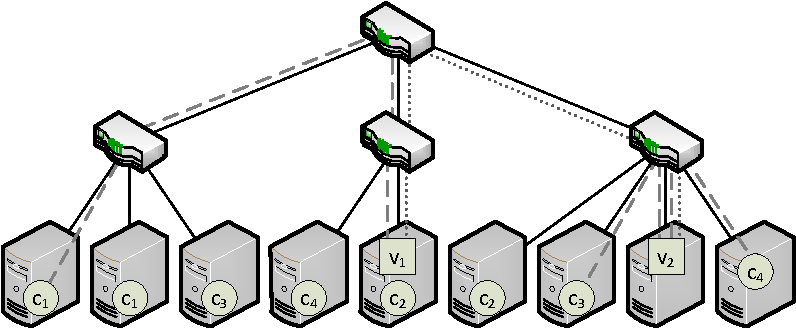
\includegraphics[width=0.79\columnwidth]{figs/static-mapping/data_locality_no_legend.pdf}
\caption{Overview: a 9-server data center storing~$\tau=4$ different chunks~$\{c_1,\ldots,c_4\}$ (depicted as \emph{circles}), each having two replicas. The replicas need to be selected and assigned to the two
 virtual machines~$v_1$ and~$v_2$; the virtual machines are depicted as \emph{squares}, and
 the network connecting them to chunks (using bandwidth~$\CostTrans$) is \emph{dashed}. In addition, the virtual machines are inter-connected among
 each other using bandwidth~$\CostCom$ (\emph{dotted}). The objective of the embedding algorithm is to minimize the overall bandwidth allocation.}\label{fig:overview}
\end{figure}


\parag{Optimization Objective.} 
Our goal is to design algorithms that minimize the resource \emph{footprint}, the most common objective function considered in the literature \cite{fischer-survey}.
%Formally, let~$\dist(v,r)$ denote the~distance (in the underlying physical network~$\Tree$) between a~node~$v$ and
%a chunk replica~$r$, and let~$\dist(v_1,v_2)$ denote the distance between the two nodes~$v_1$ and~$v_2$.
Formally, let~$\dist(v_1,v_2)$ denote the distance in the underlying physical network~$\Tree$ between the two nodes~$v_1$ and~$v_2$.
For each chunk $c$,
$\mu(c)$ is the node to which chunk $c$ is assigned,
$c^*$ is the replica of $c$ selected for processing,
and $\dist(c) = \dist(\mu(c), c^*)$, i.e., denotes the distance between active replica of chunk $c$ and the node to which $c$ is assigned.
The objective is to minimize the footprint of the virtual network, defined as follows
$$
\underbrace{\sum_{c \in C} \CostTrans \cdot \dist(c)}_{\text{chunk access cost}} +  \underbrace{\frac{1}{2} \cdot \sum_{v\in V} \sum_{v' \in \VirtualNodes\setminus\{v\}} \CostCom \cdot \dist(v,v')}_{\text{node inter-connect cost}}\enspace.
$$
The solution must obey the capacity of the substrate network: (1)~the total number of nodes hosted at each server $s$ must not exceed $\capacity(s)$, and (2)~the total bandwidth allocated at each link $e$ must not exceed its capacity $\capacity(e)$.
%Finally, the solution must assign every chunk to some node, i.e., $\bigcup_v \mu(v) = \{ c_1, \ldots, c_{\tau} \}$.

\subsection{Problem Decomposition}

We introduced the $\CTE$ problem in its full generality.
To fully chart the algorithmic complexity of $\CTE$, we decompose the problem into its fundamental components that can be activated or deactivated independently of each other, and we consider all possible variants.
Concretely, we consider $5$ aspects of $\CTE$, namely multiple chunk assignment ($\MA$),
replica selection ($\RS$), flexible node placement ($\FP$), node inter-connect ($\NI$),
and bandwidth constraints ($\BW$), as~described below.

\parag{Multiple Assignment ($\MA$).}
In most applications, the number of chunks~$\tau$ is larger than the number of nodes, and the objective is to assign multiple chunks to each node.
In each variant (regardless of $\MA$), we investigate assignments that balances chunks among nodes, i.e., where the number of chunks is divisible by the number of nodes, and each node has an~identical integer number of chunks assigned.
We require that the number of chunks assigned to each node is equal to~$\MaFactor = \tau / n_V$, and we call $\MaFactor$ the multi-assignment factor.
If the number of chunks exceeds the number of nodes, i.e., $\MaFactor > 1$, then we refer to such scenario as $\MA$.
In~the~$\CTE$ variant without $\MA$, each node has exactly one chunk assigned, i.e., $\MaFactor = 1$.

\parag{Replica Selection ($\RS$).}
Distributed filesystems often utilize data redundancy for corruption detection and correction.
A redundant data chunk has multiple \emph{replicas}, stored on different physical machines.
For each data chunk, it is sufficient to assign only one of its replicas.
By~$\RS$ we denote the flexibility of choosing which replica of each data chunk to assign.
In~the~problem variant without $\RS$, each chunk has a single replica ($r_i = 1$ for all $i$).

\parag{Flexible Placement ($\FP$).}
%In most applications, nodes of virtual network are unconcerned about their physical placement.
By $\FP$ we denote the flexibility of assignment of nodes to~physical machines.
In the problem variant without $\FP$, the assignment of nodes to physical machines is given as an input.

\parag{Node Inter-Connect ($\NI$).}
In some computational tasks, it is sufficient to process data chunks independently of each other.
However, more often the result of processing the individual chunks is combined afterwards.
By $\NI$ we refer to the latter scenario, where the computation requires the nodes to cooperate.
We investigate the scenario, where we reserve a bandwidth of volume $\CostCom$ between each pair of nodes, i.e., the node inter-connect is modelled as a complete graph, to account for the all-to-all communication patterns of batch processing applications such as MapReduce.
In the problem variant without $\NI$, we optimize only the cost of assigning chunks to nodes, and the inter-node communication is set to zero, i.e., $\CostCom = 0$.

\parag{Bandwidth Capacities ($\BW$).}
We distinguish between an uncapacitated and a capacitated scenario where each link $e$
of the substrate network comes with a bandwidth
constraint $\capacity(e)$, and we refer to the bandwidth-constrained version by~$\BW$.
Note that capacity constraints introduce infeasible problem instances, where it is impossible to
allocate sufficient resources to~embed the virtual network.
In the problem variant without $\BW$, each link has infinite capacity, i.e., $\capacity(e) = \infty$ for each edge $e$.

\section{Polynomial-Time Algorithms}\label{sec:poly}


Despite the various degrees of freedom in terms of embedding and replica selection,
we can solve many problem variants efficiently.
 This section introduces three general techniques,
 which can roughly be categorized into
 \emph{flow} (Section~\ref{ssec:flow}), \emph{matching} (Section~\ref{ssec:match}) and \emph{dynamic programming}
 (Section~\ref{ssec:dyn}) approaches.
In Figure~\ref{fig:venn_full}, we marked either the fastest method to solve the computational problem or its computational intractability.
 
First, let us make a simplifying observation:
\begin{obs}\label{obs:nofp}
In $\CTE$ variants without flexible placement (FP),
the bandwidth required
for the inter-connect network (NI) can be allocated upfront, 
as it
does not depend on the replica
selection and the assignment.
Accordingly, we can reduce the $RS+MA+NI+BW$ variant (as well as all its subproblems)
to~$RS+MA+BW$ (resp.~its subproblems).
\end{obs}

\begin{figure}[t]
\centering
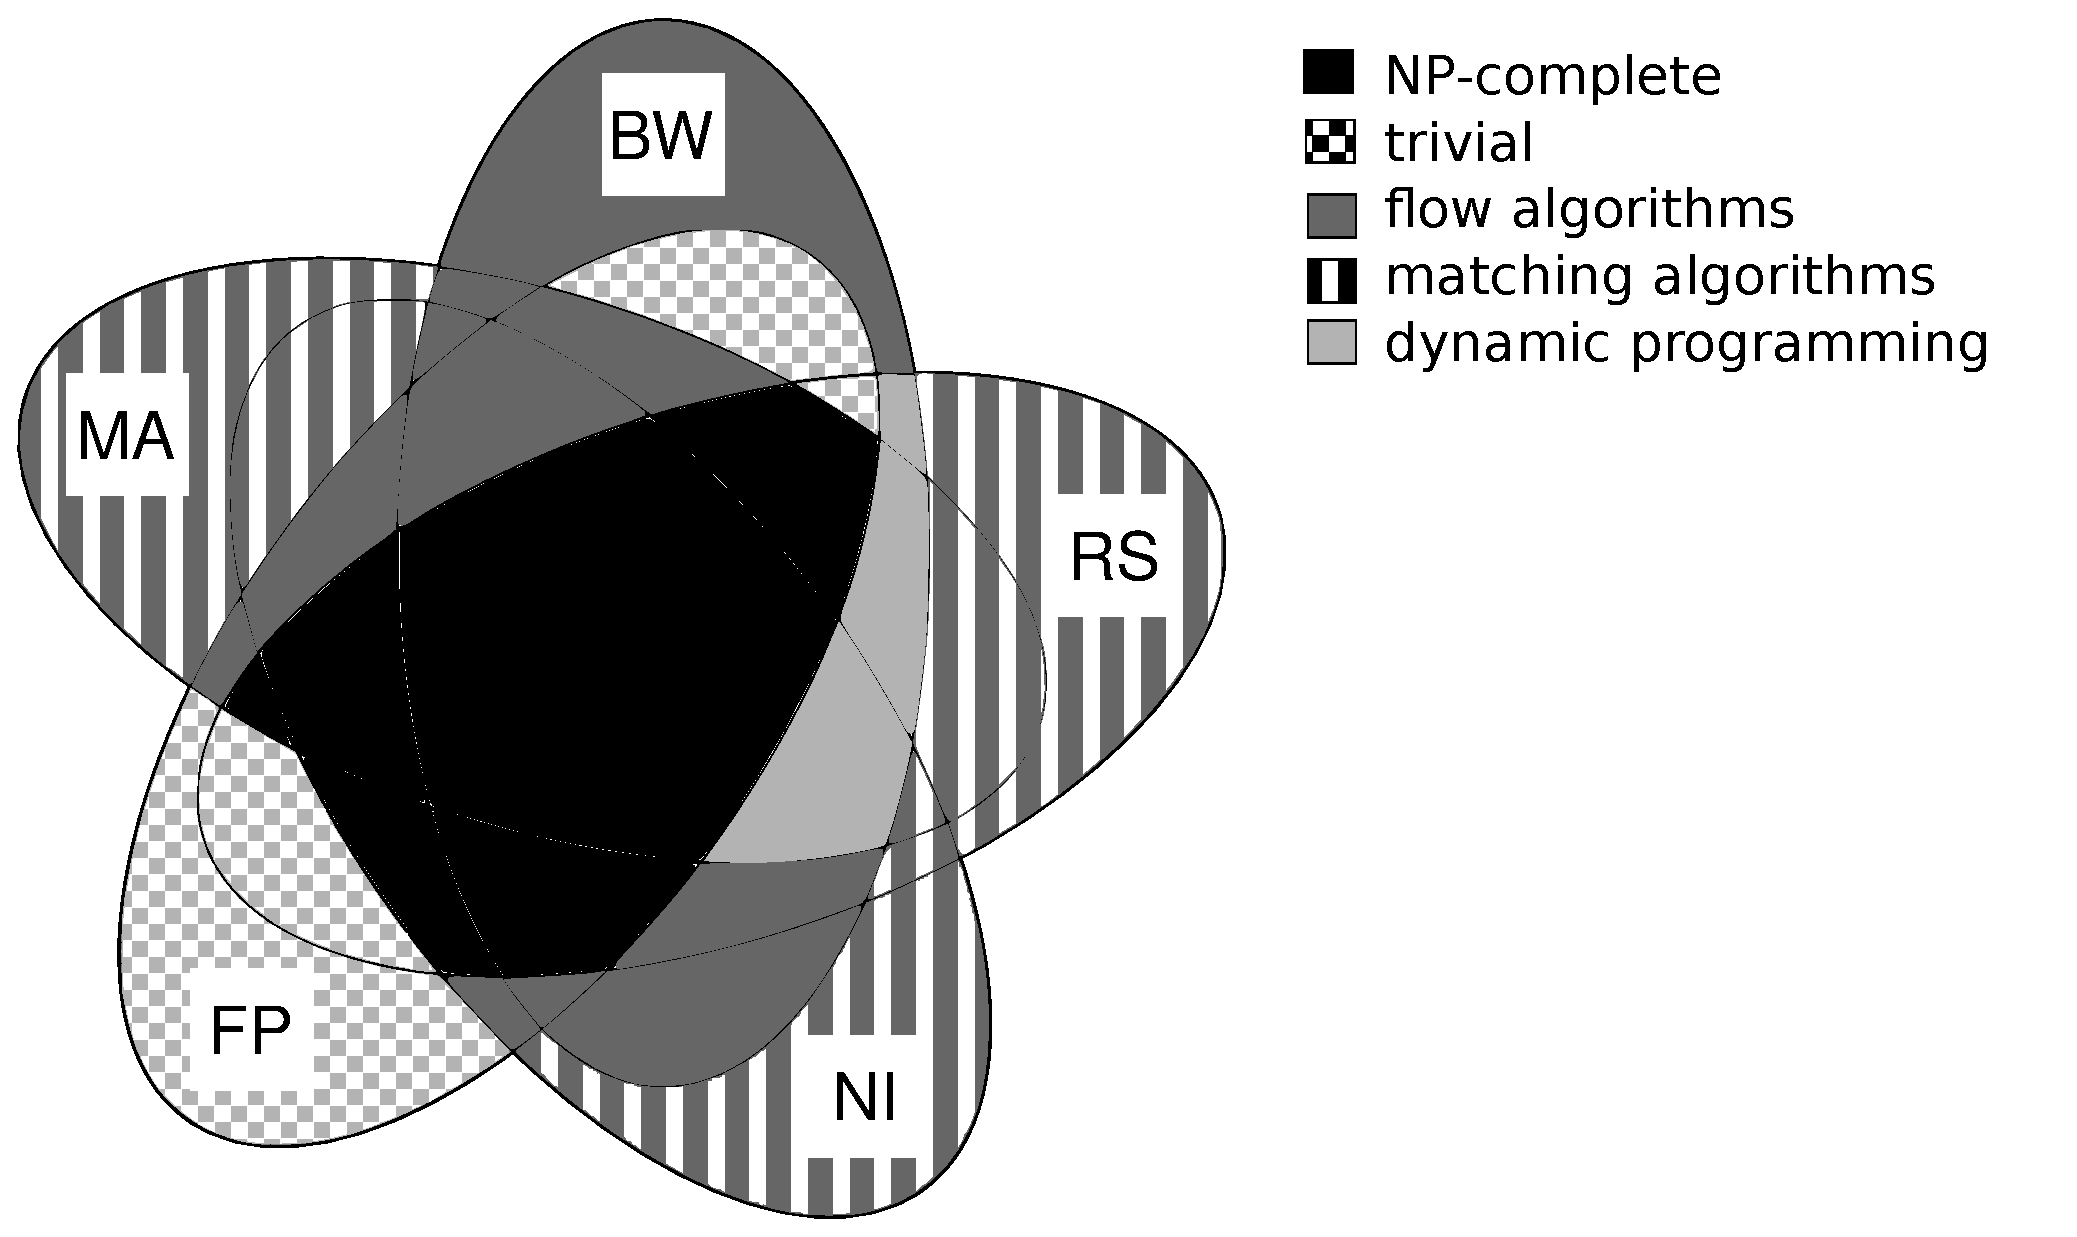
\includegraphics[width=0.69\columnwidth]{figs/static-mapping/venn_full2}
\caption{Fastest algorithms for different respective variants. Variants depicted by solid black are NP-hard, and variants depicted by checked filling are trivially solvable. For the remainder of variants we marked the fastest method.}
\label{fig:venn_full}
\end{figure}


\subsection{Flow-Based Algorithm}\label{ssec:flow}

\begin{figure}
\centering
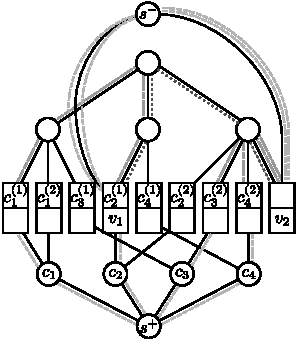
\includegraphics[width=0.5\columnwidth]{figs/static-mapping/flow_ma_cv}
\caption{An example of the extended substrate
network~$\Tree^*$: The sink~$\Sink$ is connected to the two leaves that host the
nodes. The artificial nodes are depicted below the leaves, are labeled with
their respective chunks (e.g.,~$\achunk_1$), and are connected to the source
$\Source$ as well as to the leaves that contain replicas of their chunk.
The~maximum flow with minimum cost is indicated by the dashed lines: each line
represents one unit of flow. The~dotted lines indicate links which have reduced
capacity due to~$\NI$.}
%\caption{Example of flow construction: Problem instance with two nodes, four chunk
%types, and two replicas per type. The min-cost-max-flow
%is indicated by the dashed lines: each line represents one unit of flow.
%}
\label{fig:flow_construction}
\end{figure}



%\begin{figure}[t]
%\centering
%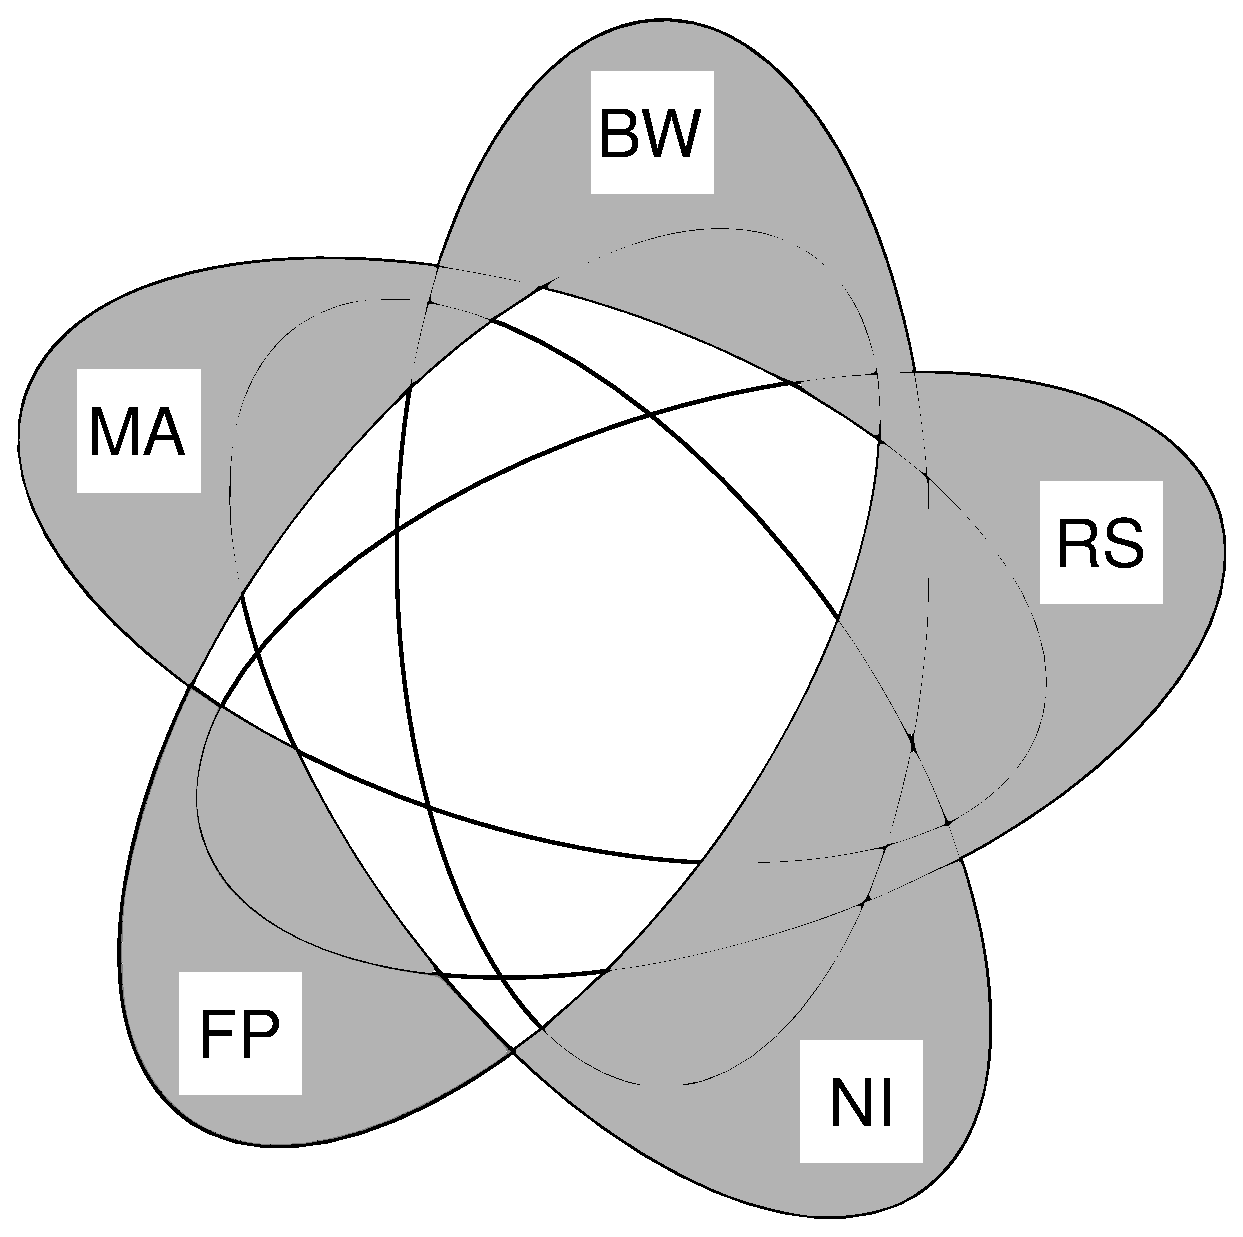
\includegraphics[width=0.49\columnwidth]{figs/static-mapping/venn_flow.pdf}
%\caption{Variants solved by flow approach.}
%\label{fig:venn_flow}
%\end{figure}


We first present an algorithm to solve the~$\RS+\MA+\NI+\BW$ variant of the $\CTE$ problem.
Recall that in this problem variant,
we are given a~set of redundant chunks ($\RS$) and a~set of
nodes
at fixed locations (no~$\FP$). The number of chunks may be larger than the number
of nodes ($\MA$), and each node needs to be connected
to its selected chunks as well as to other nodes ($\NI$), while respecting
capacity constraints ($\BW$).
As we see in the following, we can use a flow approach to solve this
problem variant.


\parag{Construction of the Artificial Graph.}
In order to solve the~$\RS+\MA+\NI+\BW$ variant of the {\CTE} problem,
we first remove the~$\NI$ component using Observation~\ref{obs:nofp}.
Then, we construct
an artificial graph~$\Tree^*$, extending the substrate network~$\Tree$.
We transform bandwidth capacities, so that they correspond to the maximal number of chunks that we can transfer through the link.
Concretely, for each link~$e\in E(\Tree)$, we set its new
capacity in~$\Tree^*$ to~$\lfloor\capacity(e) / \CostTrans\rfloor$.
After this normalization, we extend the topology of~$\Tree$ by
introducing an artificial vertex for each of $\tau$ chunks. Each of these artificial
vertices is connected to each leaf (i.e., server) in~$\Tree$ where a~replica
 of the respective chunk is located,
connecting the replica by a link of capacity~$1$. In
addition, we construct a
\emph{super-source}~$\Source$, and connect it to each of the artificial chunk
vertices with a link of capacity~$1$. Moreover, we construct an artificial \emph{super-sink}~$\Sink$ and
connect it to every leaf containing at least one node; the link capacity represents
the number of nodes this server hosts times the~multi-assignment factor
$\MaFactor$.
We additionally assign the following costs to edges of~$\Tree^*$:
every edge of the original substrate network costs one unit, and all other artificial edges
cost nothing.
A solution to the~$\RS+\MA+\BW$ variant can now be computed
from a~solution to the \emph{min-cost~max-flow} problem between super-source
$\Source$ and
super-sink~$\Sink$ on the artificial graph~$\Tree^*$.
An illustration of this construction is presented in Figure~\ref{fig:flow_construction}.

\parag{Algorithm.}
Our algorithm to solve the~$\RS+\MA+\NI+\BW$ variant consists of three parts:
First, we construct the extended graph~$\Tree^*$
described above and compute
a~min-cost~max-flow solution.
State-of-the-art~min-cost max-flow algorithm is the double scaling algorithm~\cite{mincostmaxflow-state}, which is based on the scaling technique~\cite{mincostmaxflow-1,mincostmaxflow-2}, .

Second, we have to \emph{round} the resulting, possibly fractional flow, to
integer values. Due~to the~\emph{integrality theorem}~\cite{flow-book},
there always exists an optimal integer solution on graphs with integer capacities.
However, min-cost~max-flow algorithms may yield fractional solutions
which need to be rounded to integral solutions (of the same cost)~\cite{electric-flows}.

Third, given an integer min-cost~max-flow solution, we need to decompose
the integer flow into paths
representing matched chunk-node pairs:
The assignment can be obtained by decomposing the flow allocated in the
original substrate network. In order to identify a chunk-node assignment,
we take an~arbitrary (loop-free) path~$p$ carrying a flow of value at least~$1$ from~$\Source$ to~$\Sink$:
the first hop represents the chosen chunk, the second hop the chosen
replica, and the penultimate hop represents the server: we assign
the replica to an arbitrary node on this server that has less than $\MaFactor$ chunks assigned.
Having found this pair, we reduce the flow
along the path~$p$ by one unit.
We continue the pairing process until every chunk is assigned.

\parag{Analysis.}
The runtime of our algorithm consists of four parts: construction of~$\Tree^*$,
computation of the min-cost~max-flow, flow rounding, and decomposition. The
dominant term in the~asymptotic runtime is the flow computation.
Using the double scaling algorithm for min-cost~max-flow~\cite{mincostmaxflow-state}, we get a runtime of~$\mathcal{O}(|E|^2 \cdot\log\log U \cdot \log |E|)$
where~$|E| = \mathcal{O}(n_S+\sum_{i=1}^\tau r_i + n_V)$ is the number of $\Tree^*$ edges, and~$U$ is the maximal link capacity. Note that in networks with high capacity
and uncapacitated networks, we can simply set~$U=\tau$, so the resulting overall runtime is $\mathcal{O}(|E|^2 \cdot\log\log \tau \cdot \log |E|)$.
The algorithm has a quadratic dependence on the size of substrate network $n_S$, and in next section we propose an alternative algorithm with linear dependence on~$n_S$.


\subsection{Matching Algorithms}\label{ssec:match}


%\begin{figure}[t]
%\centering
%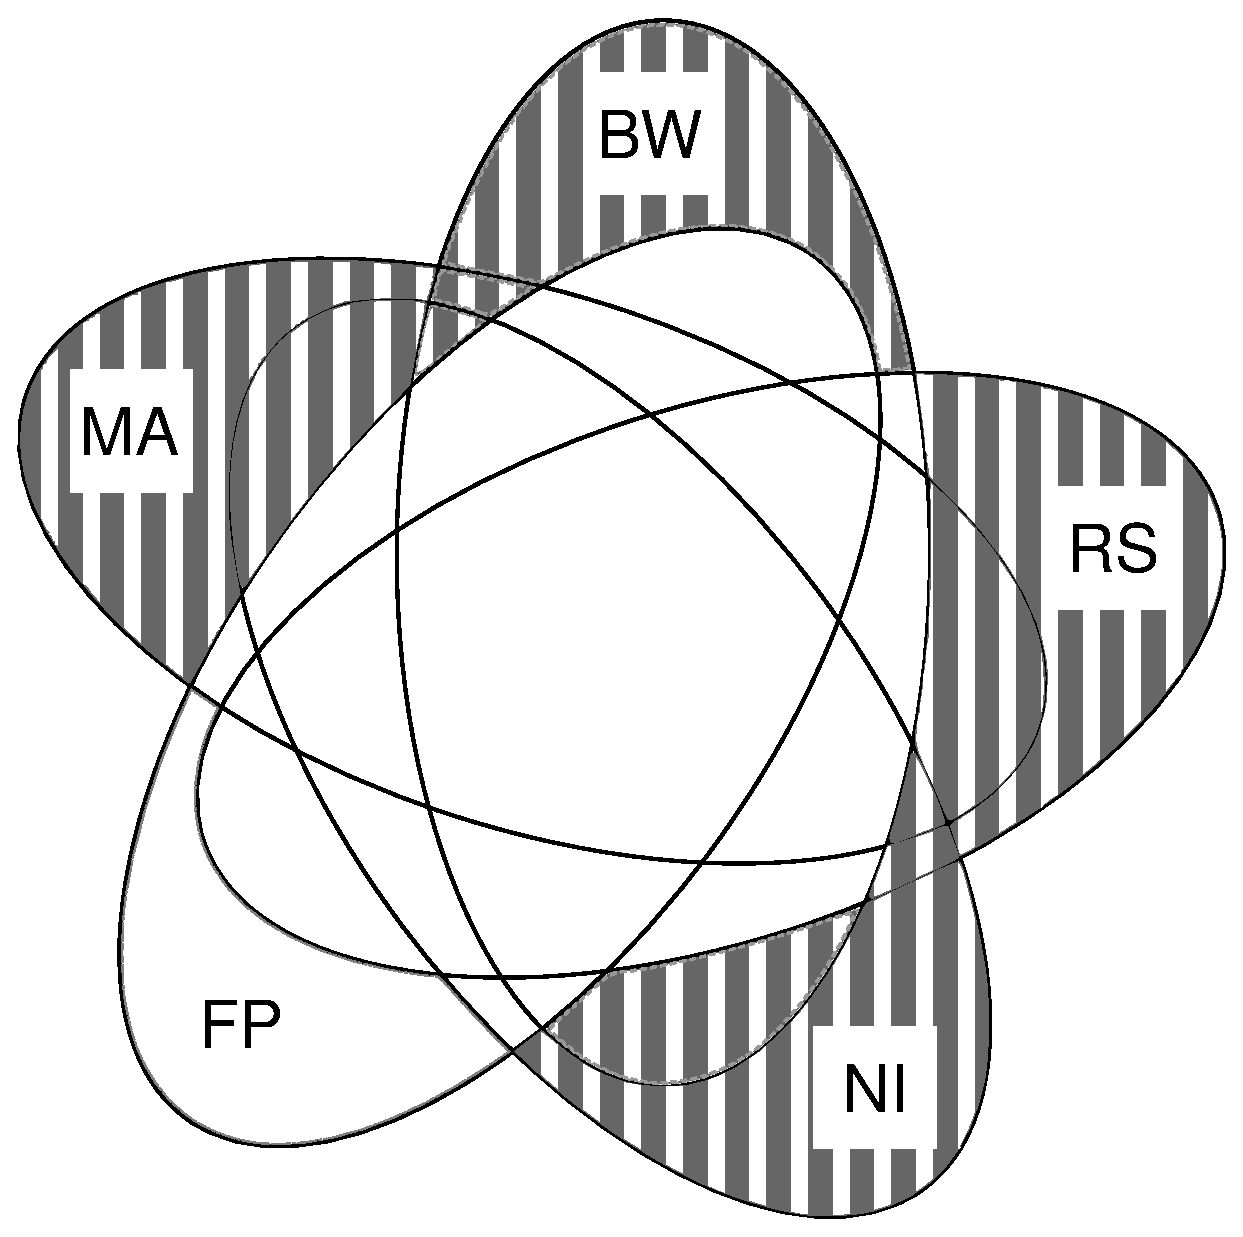
\includegraphics[width=0.49\columnwidth]{figs/static-mapping/venn_matching.pdf}
%\caption{Variants solved by matching approaches.}
%\label{fig:venn_match}
%\end{figure}
This section presents an alternative algorithm to solve $\RS+\MA+\NI$ and~$\MA+\NI+\BW$
variants of the $\CTE$ problem.
First, we consider the~$\RS+\MA+\NI$ variant.
Recall that in this variant,
we are given a~set of redundant chunks ($\RS$) and a~set of nodes
at fixed locations (no $\FP$). The number of~chunks may be larger than the number
of nodes ($\MA$), and each node needs to be connected
to its chunks as well as to other nodes ($\NI$).

\parag{Algorithm.} Due to Observation~\ref{obs:nofp}, the $\RS+\MA+\NI$ variant degenerates to~$\RS+\MA$.
In order to solve the latter,
we construct a bipartite
graph between the set
of nodes and
the set of chunks.
First, we clone each node~$\MaFactor$ times
as each node needs to assign
$\MaFactor$ chunks, and we aggregate all replicas of a given chunk in a
single %$\ChunkType$
super-vertex.
Second, we link (cloned) nodes to (aggregated) replicas.
In instances without $\BW$, assigning any replica to any node is feasible, and hence, for a given assignment $\mu$ of chunks to nodes, the minimum bandwidth is utilized if for each $c$, node $\mu(c)$ serves the closest replica of $c$.
Therefore, for each node $v$ and chunk~$c$, we connect each copy of $v$ and the super-vertex $c$ with the link of cost $\min_i \dist(v,c^{(i)})$, i.e., the cost of reaching the closest replica.
Finally, on the resulting bipartite graph, we compute a~\emph{minimum weight
perfect
matching}:
the resulting matching describes the optimal assignment of chunks to nodes.
An example instance is presented in Figure~\ref{fig:matching}.


\begin{figure}
  \centering
  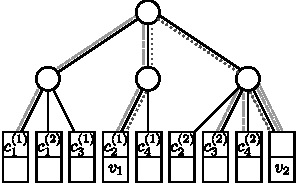
\includegraphics[width = 0.39\columnwidth]{figs/static-mapping/model_ma_r_cv_boxes}
  \centering
  \hspace{1cm}
  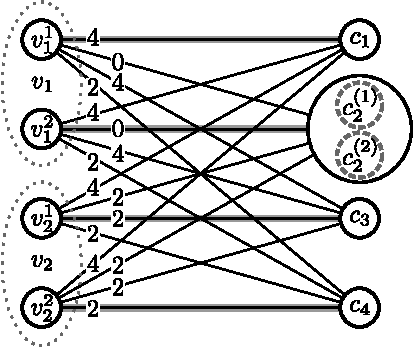
\includegraphics[width =0.39\columnwidth]{figs/static-mapping/matching}
\caption{The~$\RS+\MA$ variant on the left is converted into a
  matching problem instance on the right.
The figure illustrates
an instance where two nodes are
cloned into~$\MaFactor = 2$ nodes each,
resulting in a total of four nodes in
the matching representation.
The two replicas of each chunk~$\achunk_j$ are
aggregated into a single super-vertex  in the matching instance, and
this gives a total of four super-vertices in the matching graph.
%The costs
%on the links between all clones of a specific vertex and a chunk are set to
%the minimum distance. For instance, the weights of edges connecting
%the two clones of~$\VirtualNode_1$ to~$\achunk_2$ are 0.
}
\label{fig:matching}
\end{figure}

\parag{Analysis.}
The runtime consists of two parts: the construction of the matching graph and
the~actual matching computation. The constructed graph consists of
$(\MaFactor \cdot n_V) \cdot \ChunkType = \tau^2$
many edges,
and for each edge we compute its weight. The shortest distances
in a tree of size $n_S$ can be computed in time~$\mathcal{O}(n_S + q)$~\cite{offline-lca}, where $q$ is the number of queried pairs, which translates to the overall construction time~$\mathcal{O}(n_s + n_v\cdot \sum_{i=1}^\tau r_i)$.
The state-of-the-art algorithm to compute matchings in bipartite graph~\cite{matching-best} has a running time of $\tilde{\mathcal{O}}(|E|^{10/7}\cdot \log W)$, where $|E|$ is the number of edges, $W$ is the maximum weight of an edge, and $\tilde{\mathcal{O}}$ hides polylogarithmic (in terms of $|E|$) factors.
The total running time is then $\tilde{\mathcal{O}}(\tau^{20/7}\cdot \log(n_s)) + \mathcal{O}(n_s + n_v\cdot \sum_{i=1}^\tau r_i)$.
Note that the matching-based algorithm has a linear dependence on the size of the substrate network~$n_S$, whereas the flow-based algorithm runtime contains the term $\mathcal{O}(n_S^2)$.


\subsubsection{Local matching algorithm}

Now, we present the way to solve the~$\MA+\NI$ variant even faster by using greedy approach.
Moreover, we show that we can
even solve
$\MA+\NI+\BW$ variants by simply
verifying feasibility.
In~the~following, due to Observation~\ref{obs:nofp}, we can focus on
the~$\MA$ and~$\MA+\BW$ variants, respectively.
We start by lower-bounding the required bandwidth allocation.
The \emph{uplink} of a~proper subtree $T'$, denoted $\Uplink(T')$ is an edge from the root of $T'$ to its parent.

%We first introduce the following definition.
%\begin{defn}[Local Assignment (LA)]\label{def:loc}
%We define an assignment~$\VmChunkAssignment$ to
%be \emph{local in a specific subtree~$\Tree'$}, iff~$\VmChunkAssignment$
%assigns the maximum number of chunks in the
%subtree to nodes in the same subtree.
%We define~$\VmChunkAssignment$ to be \emph{local} when
%it is local with respect to all possible subtrees of the~substrate network.
%\end{defn}
%
%\begin{figure}
%\center
%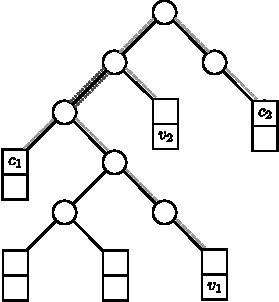
\includegraphics[width = 0.45\columnwidth]{figs/static-mapping/unbalanced_tree}
%\caption{Illustration of local assignment: The dashed lines indicate bandwidth allocations, which occur
%independently of the chosen assignment. The dotted lines indicate bandwidth
%allocation which occur only if~$c_2$ is assigned to~$v_1$.}
%\label{fig:unbalanced_tree}
%\end{figure}
%
%\parag{Example.}
%Figure \ref{fig:unbalanced_tree} illustrates the concept of local assignment:
%The closest chunk to~$v_2$ is~$c_1$, and the closest node to~$c_1$ is~$v_2$.
%However, a subtree~$T'$ exists such that~$v_1 \in T'$ and~$c_1
%\in T'$, but~$v_2 \notin T'$. Therefore, a local assignment cannot assign~$c_1$ to~$v_2$.


%Later we will see that
%optimal solutions to
%$\MA$ have a local assignment. We exploit this in our algorithms described
%in the following.


\begin{lemma}\label{lem:uplink-alloc}
In the~$\MA$ variant of $\CTE$, a proper subtree~$\Tree'$
containing~$\tau(T')$
chunks and $x$~nodes, the bandwidth allocation on the uplink of $\Tree'$ is at~least ${\CostTrans\cdot|\tau(T')-x\cdot\MaFactor|}$.
\label{lemma:uplink}
\end{lemma}
\begin{proof}
In case the number of chunks equals the processing capacities of the
nodes in the given subtree,
the bandwidth allocation inflicted by the chunk access network on the uplink is zero, since we can assign all chunks to nodes in the same subtree.
Otherwise, we distinguish between two cases. If there are more chunks in the subtree, at least all excess chunks have to
be assigned to nodes outside $T'$, which 
inflicts costs~$\CostTrans$ per excess chunk on the uplink of~$\Tree'$.
 Similar situation occurs if the processing capabilities exceed the
amount of
available chunks.
Hence, the minimum bandwidth allocation for the chunk access on the uplink
is the absolute difference between the number of chunks and the processing capabilities
of the subtree, i.e.,~$|\tau(T')-x\cdot\MaFactor|$ times $\CostTrans$.
\end{proof}


\parag{Algorithm.} Our proposed algorithm for the $\MA$ variant of $\CTE$
proceeds in a bottom-up fashion, traversing the~substrate network~$\Tree$
from the leaves toward the root.
For each subtree~$\Tree'$, we maintain
two sets~$S_c,S_v$ in order to map unassigned
chunks~$S_c$ in the subtree~$\Tree'$ to 
nodes~$S_v$ in~$\Tree'$. Both sets are initially empty.
We associate a counter with each node that enters $S_v$, and we initialize it to $\MaFactor$, the multi-assignment factor.


We first process all the leaves, in an arbitrary order; subsequently, we process inner vertices
of~$\Tree$ whenever all their children have been processed.
We process any leaf~$\ell$
by adding any
nodes or chunks which are located on~$\ell$ to the corresponding sets~$S_c$ and~$S_v$.
A non-leaf vertex~$u$ is processed in the following way: we take the union of
the sets corresponding to~$u$'s children, i.e., the sets containing the unmatched chunks and nodes
in this subtree.
For both leaves and inner nodes, whenever
both sets are non-empty, we greedily assign an arbitrary chunk $c$ in~$S_c$ with an arbitrary node $v$ in~$S_v$.
Then, we remove $c$ from $S_c$, and we decrement the counter of $v$. If the counter of $v$ reaches zero, we remove $v$ from $S_v$.

\parag{Analysis.} For each
vertex in the substrate graph,
we build the union of the
children's sets.
The number of all remove operations is equal to
the number of chunks~$\mathcal{O}(\ChunkType)$.
Hence the overall complexity of this construction amounts to
$\mathcal{O}(n_S + \ChunkType)$.
The local matching algorithm outperforms the previous algorithm that relied upon calculating the minimum-weight perfect matching.

%It remains to prove optimality of such local assignments.
%By \emph{uplink} of a subtree with root $r$ we denote the edge from $parent(r)$ to $r$ (if it exists).
%We first characterize the bandwidth allocation on uplinks of subtrees.

%\begin{theorem}
%Given an~$\MA+\NI$ variant instance, a feasible assignment~$\VmChunkAssignment$
%is optimal iff it is local.
%\label{thm:local_optimal}
%\end{theorem}
%
%\begin{proof}
%Local assignments generate exactly the minimal allocations on all links, as
% the assignments which generate the minimal bandwidth allocations
%described in
%the proof of
%Lemma~\ref{lemma:uplink} are local in the given subtree. Hence
%each local assignment has to be optimal. A non-local assignment, has at least
%one subtree, in which it is not local. This subtree has a higher
%allocation on the uplink. Since the local assignment has minimal allocations
%on all other links, the non local assignment has a larger footprint.
%\end{proof}

The algorithm allocates the minimum possible bandwidth at an uplink of every subtree, as stated in Lemma~\ref{lemma:uplink}, and hence the algorithm computes an optimal solution.
Combined with a~simple post-processing step, this approach can also solve~$\MA+\BW$ variant. The central idea of this extension is
that the algorithm allocates the minimal bandwidth
on each individual edge. In consequence, any bandwidth constraint,
lower than the requirement given in Lemma~\ref{lem:uplink-alloc}, renders
the problem infeasible. Hence, it is sufficient to temporarily omit the
bandwidth limitations, compute an optimal assignment for an~$\MA$ instance, and
verify that the resulting allocations do not violate any capacities. The
post-processing step scales linearly with the number of edges in the substrate
graph.


\subsection{Dynamic Programming}\label{ssec:dyn}

We now show how to solve the~$\MA+\FP+\NI+\BW$ variant
in polynomial time.
Note that this variant requires to find a
tradeoff between the desire to place nodes as close as possible to each other
(in order to minimize communication costs), and the desire to place nodes
as close as possible to
the chunk locations.




\parag{Example.} Figure~\ref{fig:dynamic_motivation} shows an example: one
extreme solution is to minimize the distance between chunks and nodes,
see mapping~$\NodeMapping_1$ in the left picture in
Figure~\ref{fig:dynamic_motivation}: the four nodes are all
collocated with chunks, resulting in a zero-cost chunk access network. As a
result, the paths between the individual nodes are longer than in alternative
node placements: each node has a~distance of two hops to one other node,
and four hops to two other nodes. Hence the resulting allocations for the
node inter-connect sum up to~$20 \cdot \CostCom$.

%\begin{figure}[t]
%\centering
%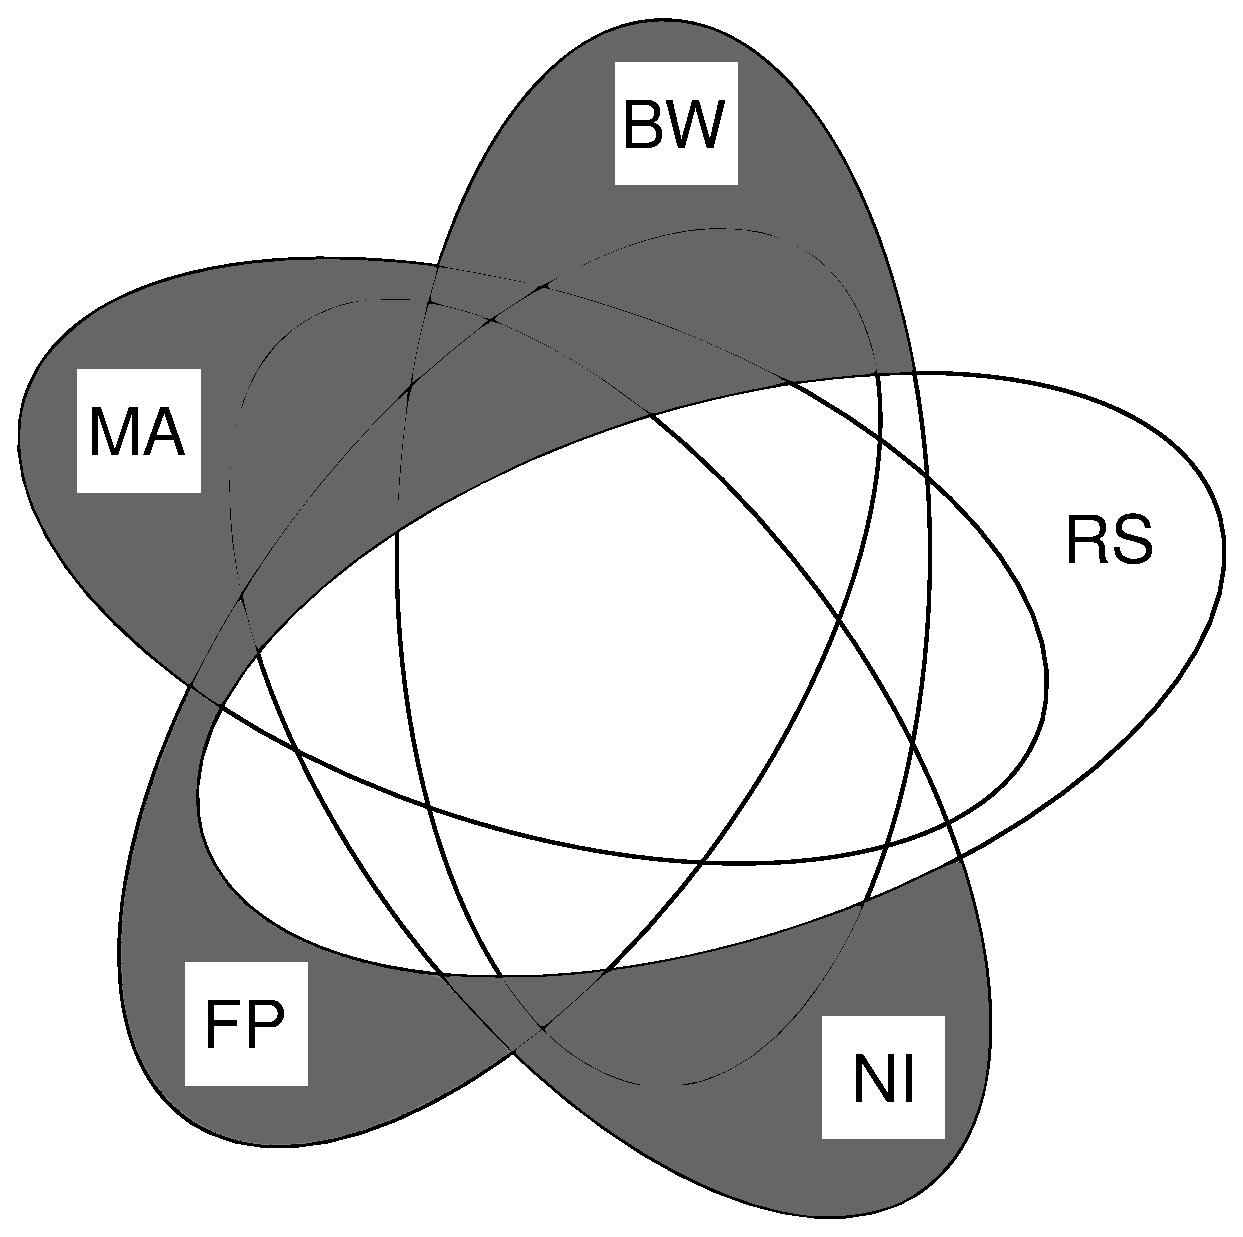
\includegraphics[width=0.49\columnwidth]{figs/static-mapping/venn_dp.pdf}
%\caption{Variants solved by dynamic programming approach.}
%\vspace{-1em}
%\label{fig:venn_dp}
%\end{figure}

The right picture in Figure~\ref{fig:dynamic_motivation} shows a different node
mapping~$\NodeMapping_2$, which seeks to minimize the inter-connect costs
between the nodes, and places all nodes in one subtree. The distance between all
nodes is $2$, which results in a total bandwidth allocation of~$12\cdot\CostCom$
for the inter-connect. However, this reduced price comes at additional costs in
the access network:~$c_3$ and~$c_4$ have to be assigned to~$v_3$ and~$v_4$,
which requires a total bandwidth allocation of~$8 \cdot \CostTrans$.


\begin{figure}
  \centering
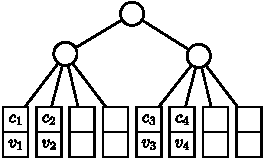
\includegraphics[width = 0.39\columnwidth]{figs/static-mapping/dynamic_bad}
\hspace{1cm}
\centering
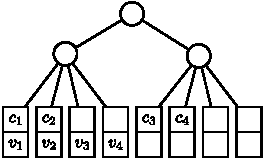
\includegraphics[width = 0.39\columnwidth]{figs/static-mapping/dynamic_good}
\caption{Two different node placements for the same substrate graph and chunk
locations. For~$\CostTrans = \CostCom$, both solutions have an identical
footprint. In other cases, one solution outperforms the other.}
\label{fig:dynamic_motivation}
\vspace{-1em}
\end{figure}



\parag{Algorithm.} Our proposed approach is based on dynamic programming, and
leverages the \emph{optimal substructure property} of the $\MA+\FP+\NI+\BW$ variant:
as we will see, optimal solutions for subtrees
can be efficiently combined into optimal solutions for the whole tree.
First, we transform the
substrate network~$\Tree$
into a binary tree:
we clone every higher-degree node,
iteratively attaching additional clones as right children
and original children as left descendants.
New edges between cloned vertices constructed during the binarization have infinite capacity.

As usual in dynamic programs, we define, over the structure of the tree, a
recursive formula~$f$ for
the minimal cost solution given any possible number of nodes
embedded in a given subtree (the actual set of nodes does not matter,
due to symmetry).
The value of $f(T', x)$ corresponds to the minimum bandwidth cost of placing $x$ nodes in a subtree $T'$.
It is defined as the bandwidth allocated inside $T$ plus the bandwidth allocated on the uplink of $T'$.
The latter is equal to
\[
bw(T',x) = 
    \CostTrans\cdot|\tau(T')-x\cdot\MaFactor| +\CostCom \cdot
(\Vms - x) \cdot x\enspace, \\
  \]
  where $\tau(T')$ is the number of chunks in a~subtree~$T'$.
  If~$bw(T',x)$ exceeds the capacity of the uplink of $T'$, we set $bw(T', x) = \infty$.
  The first term of $bw$ represents
the bandwidth necessary to transport the chunks in $T'$ from their location to
nodes outside of $T'$ (see Lemma~\ref{lemma:uplink} for similar argument).
The second term of $bw$ represents the required bandwidth for the communication between the~$x$
nodes inside~$T'$, and the~$\Vms - x$ nodes in the remaining parts of the substrate
network.
Then, the formula to calculate the function $f$ for a subtree containing only a leaf $\ell$ is
\[
f(\{ \ell \}, x) =
\begin{cases}
   \infty & \mbox{if } x > \capacity(\ell)\enspace,\\
    bw(\{ \ell \}, x) & \mbox{otherwise}\enspace. \\
  \end{cases}
  \]
We set~$f(\{ \ell \},x)$ to infinity if $x$ exceeds the node hosting capacity of server $\ell$.

To calculate the value of $f(T', x)$ for non-leaf subtree $T'$, we split $x$ nodes
into two positive integer
values $r$ and $x-r$, and we put~$r$ on the right and~$x - r$ on the left subtree.
That is, we take the optimal cost
(given recursively) of placing~$r$ nodes in
the right subtree~$\textsc{Ri}(T')$ of~$T'$ and~$x-r$ nodes in the left subtree~$\textsc{Le}(T')$ of
$T'$. Given the cheapest combination, we add the bandwidth requirements
on the uplink of~$T'$ to generate the overall costs for placing~$x$ nodes in~$T'$, obtaining
\[
  f(T', x) = 
    \min_{0\leq r \leq x} \{  f\left(\textsc{Le}(T'),
x-r\right) +
f\left(\textsc{Ri}(T'), r\right) \} + bw(T',x)\enspace.
  \]

We compute~$f$ in a bottom-up manner. 
To finally compute the actual optimal embedding,
we traverse the computed minimal-cost path backwards,
according to
the optimal values found for~$f$ during the bottom-up computation.


\parag{Analysis.}
The substructure optimality follows from the observation that
costs can be accounted on the uplink, and the fact
 that we check each possible node distribution.
For each substrate vertex ($n_S$ many) we have
to check the cost of all possible splits,
resulting in an overall complexity of~$\mathcal{O}(n_S \cdot n_V^2)$.
The runtime to binarize~$\Tree$ is asymptotically negligible in comparison.


\subsection{Simple Variants}

%\begin{figure}
%\centering
%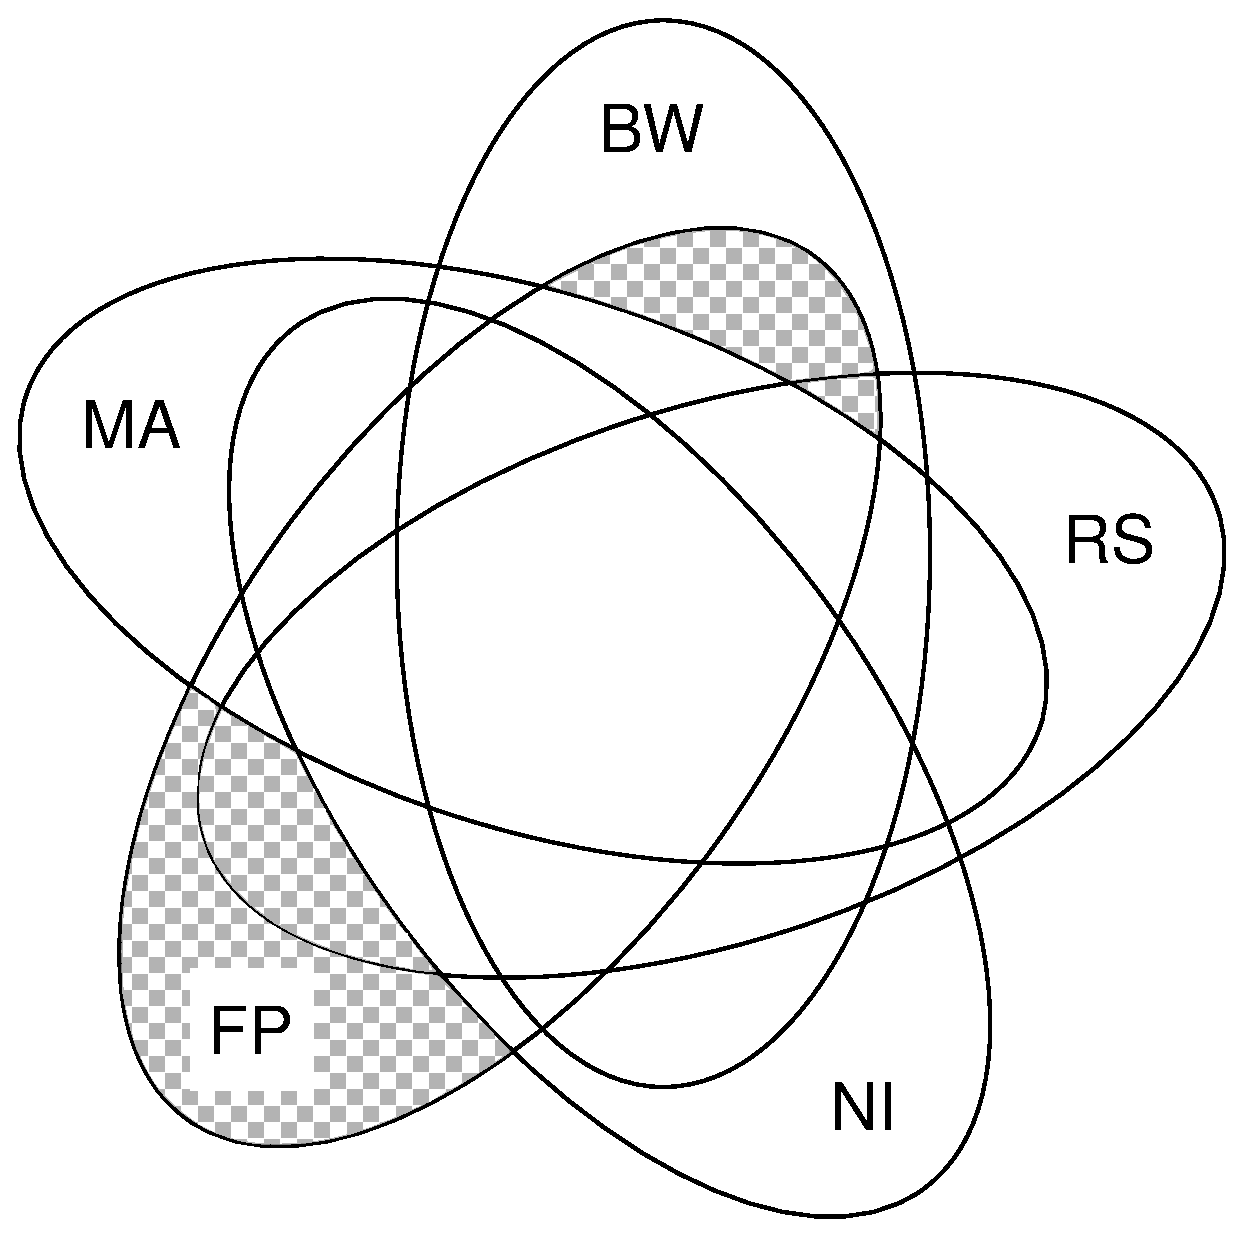
\includegraphics[width=0.49\textwidth]{figs/static-mapping/venn_trivial.pdf}
%\caption{Trivially solvable variants.}
%\label{fig:venn_trivial}
%\end{figure}


For the sake of completeness, we also observe that there are
several variants that admit a trivial solution. Concretely, variants with~$\FP$
plus any combination of
$\RS$ and~$\BW$ (but without~$\MA$ and~$\NI$) can easily be solved by
assigning
nodes to chunk locations.
%Figure~\ref{fig:venn_trivial}
%shows a Venn diagram of the trivial property combinations.

%%%%%%%%%%%%%%%%%%%%%%%%%%%%%%%%%%%%%
\section{NP-Hardness Results}\label{sec:np}

We have seen that even variants with multiple dimensions of
flexibility can be solved optimally in polynomial time.
This section now points out fundamental
limitations in terms of computational tractability.
In particular, we
show that variants become NP-hard if flexibly placeable nodes ($\FP$) have to be assigned to one of multiple replicas ($\RS$), either with multiple chunks per node ($\MA$ in Section~\ref{ssec:fprsma}) or with communication among nodes ($\NI$ in Section~\ref{ssec:fprscc}).
Both results hold even in uncapacitated networks, and even in small-diameter
substrate networks (namely two- or three-level trees).
Clearly, the hardness of the $\FP+\RS+\MA$ and~$\FP+\RS+\NI$ variants imply
the hardness of more general ones.

In addition to the hardness results for the aforementioned $\CTE$ variants, we study the influence of restricting number of replicas of a chunk on computational tractability on these variants.
Namely, we introduce the restricted replica selection component $\RS(r_{max})$, parameterized by an~integer $r_{max}$, that restricts the number of replicas of any chunk: for every chunk $c_i$ we have $r_i \leq r_{max}$.
We consider $\RS(2)$ component in relation with multi-assignment~($\MA$): we first present the NP-hardness of the unrestricted scenario $\FP+\RS+\MA$ as a warm-up,
and then we present more refined hardness result for ${\FP+\RS(2)+\MA}$.
%Finally, in Section~\ref{ssec:fprscc}, we present the NP-hardness of the unrestricted scenario $\FP+\RS+\NI$ (Theorem~\ref{theorem:fp_rs_cc}).
%However, restricted replica selection $\RS(2)$ in combination with Node-Interconnect requires additional ways to control the placement of nodes, and the NP-hardness result uses bandwidth constraints $\BW$~\cite{my-tcs}.

\subsection{Introduction to 3D Perfect Matching}
\label{sec:3dm_intro}

The hardness of both~$\FP+\RS+\MA$ and~$\FP+\RS+\NI$ variants of the $\CTE$ problem uses a reduction
from the NP-complete \emph{3D Perfect Matching} problem~\cite{3dmatch},
which can be seen as a generalization of bipartite matchings to 3-uniform
hypergraphs. We refer to this problem as~$\TDM$ and we
review it quickly for completeness.
$\TDM$ is defined as follows: we are given three finite and disjoint
sets~$X$,~$Y$, and~$Z$ of cardinality~$k$, as well as a~subset of triples~$P\subseteq
X \times Y \times Z$.  Set~$M \subseteq P$ is a 3-dimensional matching
if and only if, for any two distinct triples~$t_1=\langle x_1, y_1, z_1\rangle \in M$
and~$t_2= \langle x_2, y_2, z_2 \rangle \in M$, it holds that~$x_1\neq x_2$,~$y_1\neq
y_2$, and~$z_1\neq z_2$. The goal is to decide if there exists
a subset of triples $M \subseteq P$ that is \emph{perfect}, i.e., covers all
elements of~$X \cup Y \cup Z$ exactly once.


\subsection{Hardness of Multi-Assignments}\label{ssec:fprsma}

%\subsubsection{Warm-up: Multi-Assignment with Unrestricted Number of Replicas}
The proof of hardness of the $\FP+\RS+\MA$ variant of the $\CTE$ problem is based on the following construction.
Let~$\ITDPM$ be an instance of~$\TDM$ with $p$ triples and set cardinality~${k = |X| = |Y| = |Z|}$.
We create an instance~$\ICTE$ of the $\CTE$ problem in the following way:
\begin{enumerate}
\item \emph{Substrate network:} We construct a substrate network in a form of a tree consisting of a~root,
and for each triple from $P$, we construct a \emph{triple gadget} which we directly attach as
a child of the root. The gadget is of height 2,
and consists of an inner node and three leaves.
\item \emph{Chunks:} For each element in~$X$,~$Y$ and~$Z$,
 we construct a chunk
($3 \cdot k$ chunks in total). Every gadget contains three chunk replicas (one per leaf),
corresponding to the elements of the triple.
Note that the number of replicas for a chunk for element $e$ corresponds to the number of triples that contain $e$.
\item \emph{Other properties of the instance:}
To transform the optimization problem into a decision problem, we determine that the solution is feasible if it has a cost at most~$\Thr = 4\cdot k$ (the $\Thr$ is the acceptance threshold).
We fix the number of to-be-embedded nodes $n_V = k$,
$\CostTrans = 1$, and the the multi-assignment factor
$\MaFactor=3$.
\end{enumerate}

%\parag{Example.} Figure~\ref{fig:fprsma} shows an example of our construction: In an~instance~$\ITDPM$
%of 3-DM sets $X, Y, Z$ consist of the following elements: $X = \{ x_1, x_2 \}, Y = \{ y_1, y_2 \}$ and $Z = \{ z_1, z_2 \}$.
%Set of triples $P$ contains three triples
%$(x_1, y_1,
%z_1)$,~$(x_2, y_1, z_2)$, and~$(x_2, y_2, z_2)$. This instance has only one solution:~$M =
%\{(x_1,y_1,z_1),(x_2,y_2,z_2))\}$.
%
%To construct the corresponding instance~$\ICTE$ of the $\CTE$ problem, we
%create a gadget for each triple in~$P$. For each variable which occurs in a
%triple, the corresponding gadget contains a~chunk of the
%type of the variable. The triple
%$(x_2, y_1, z_2)$ of the instance is represented by the middle gadget in
%Figure~\ref{fig:fprsma}. The objective of~$\ICTE$ is to allocate~$k=2$ nodes
%with the smallest possible footprint. If the total footprint is at most $4\cdot k$, we can construct a solution to~$\ITDPM$ from the solution to~$\ICTE$.
%The footprint consists of the costs which occur when a node is embedded in a~gadget, and the three chunks of that gadget which are assigned to that node: one of
%the chunks is collocated with the node, the other two have to be transferred
%via two hops, incurring unit costs on each hop.


\begin{figure}[t]
  \centering
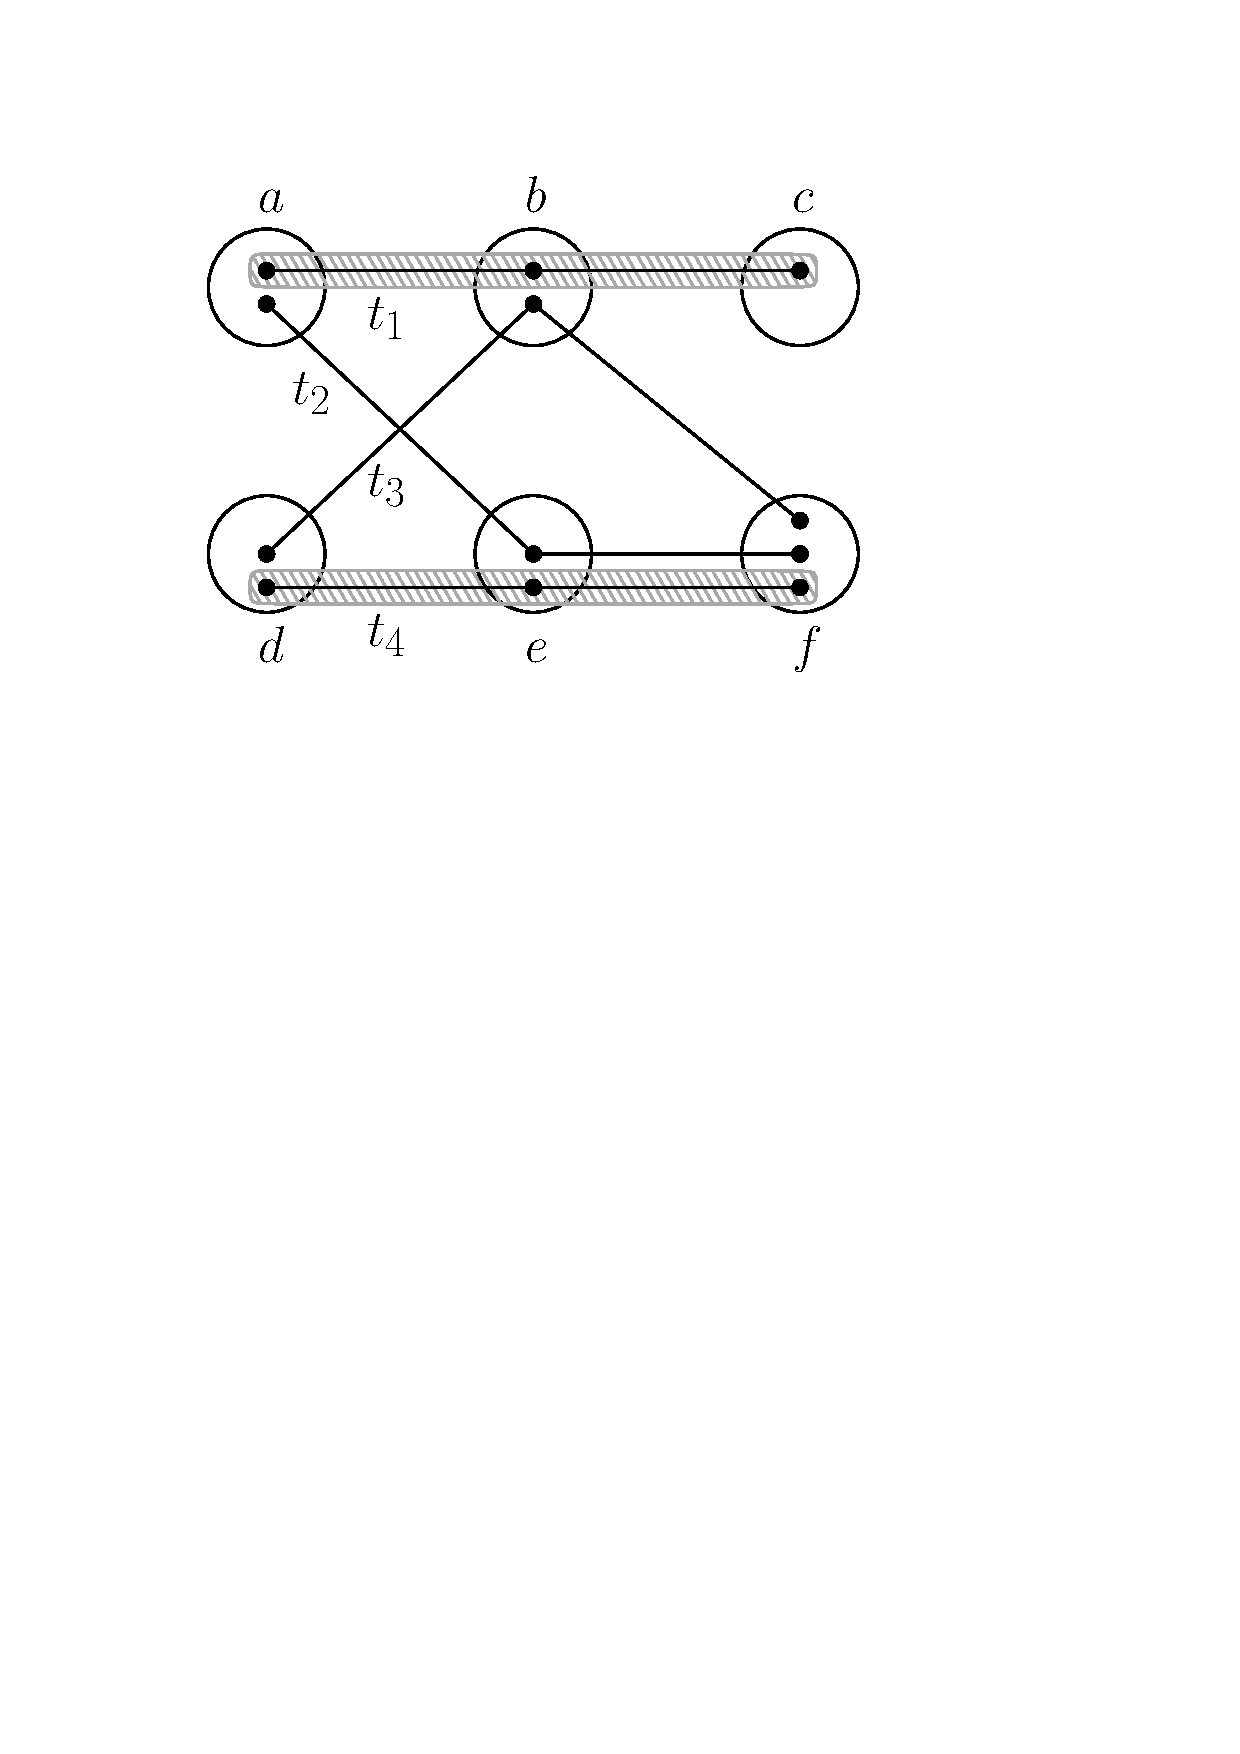
\includegraphics[width = 0.31\columnwidth]{figs/static-mapping/tdp-example}
\hspace{1cm}
\centering
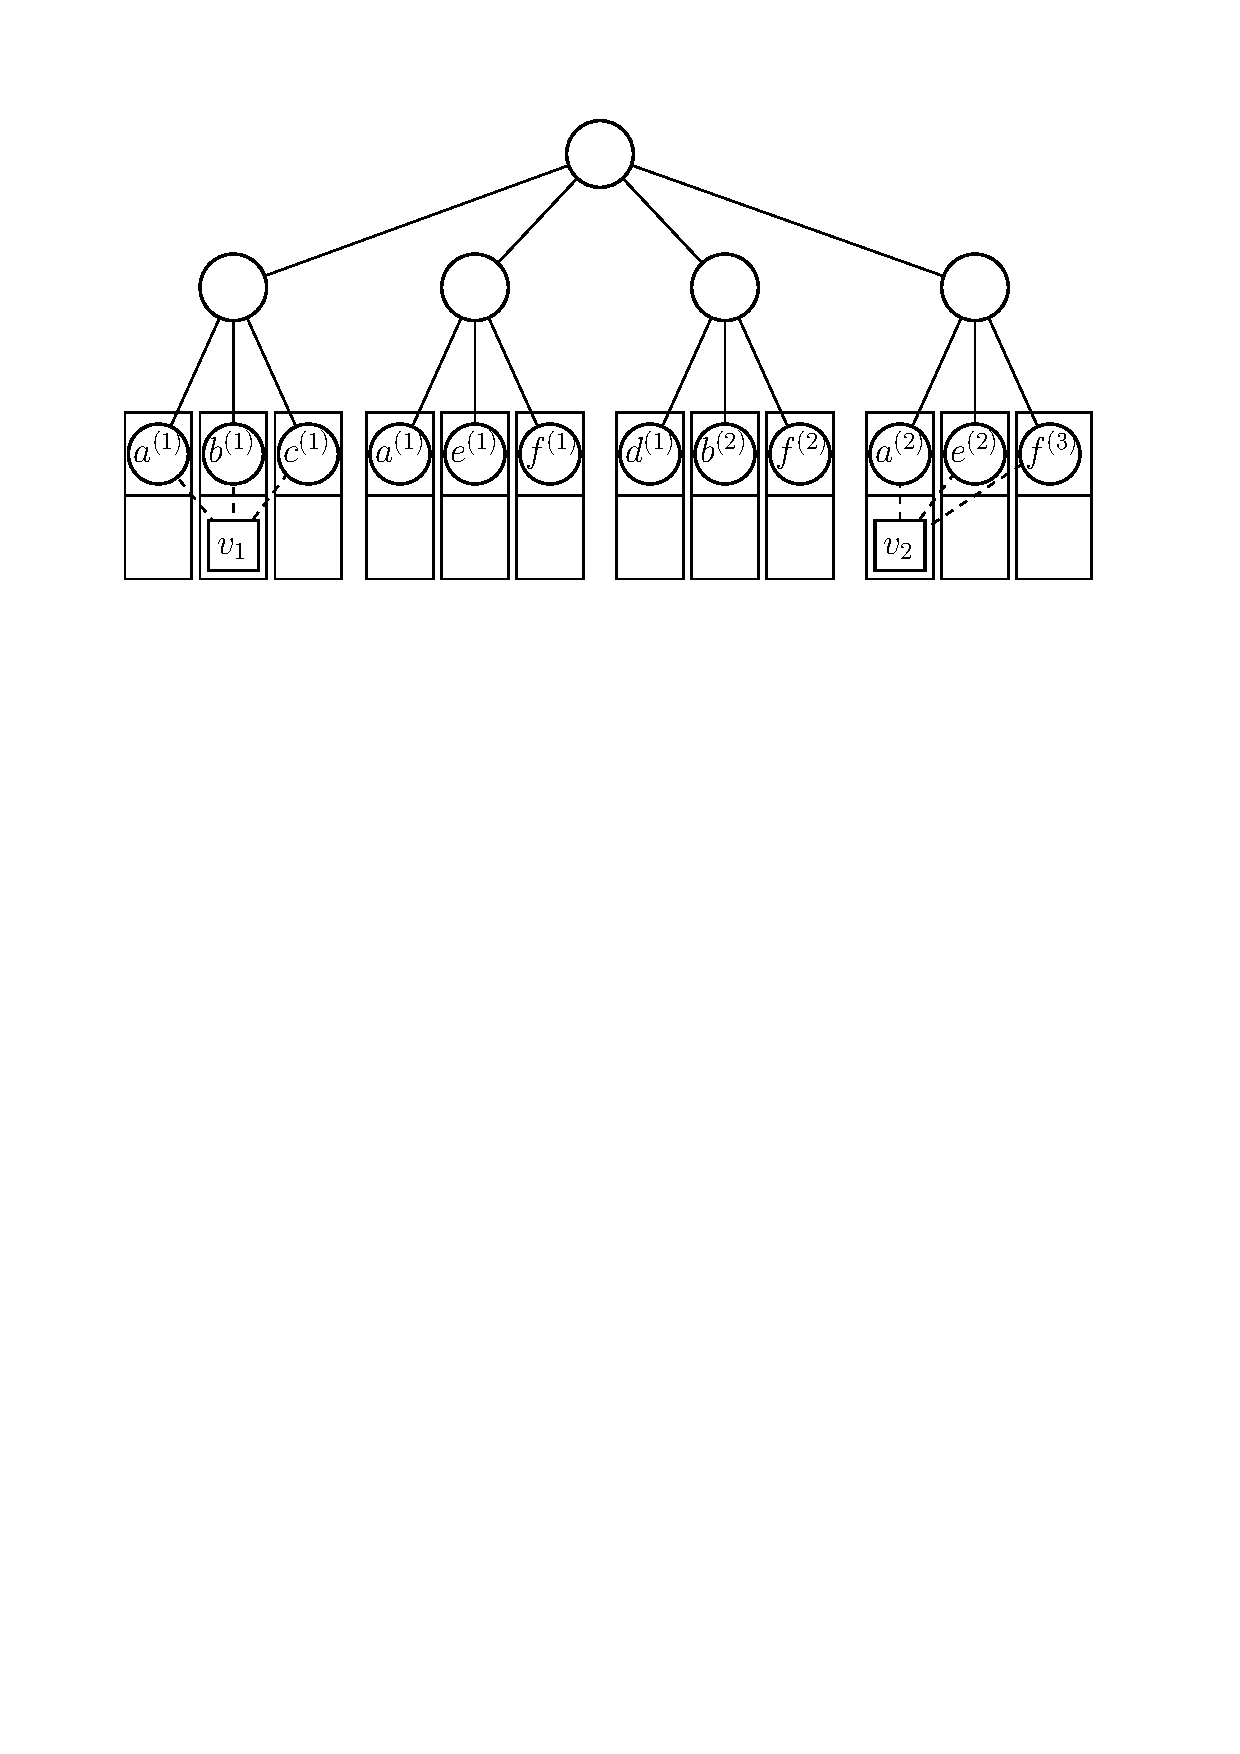
\includegraphics[width = 0.55\columnwidth]{figs/static-mapping/cte-ma}
\hfill
\caption{\textit{Left:} A~$\TDM$ instance of cardinality $k=2$ with four triples:
$t_1 = \langle a, b, c \rangle$,~$t_2 = \langle a, e, f \rangle$, $t_3 = \langle d, b, f \rangle$, and $t_4 = \langle d, e, f \rangle$. The solution is
indicated by the grey triples $t_1$ and $t_4$. \textit{Right:} The corresponding instance and an optimal solution for the~$\FP + \MA
+ \RS$ variant of the $\CTE$ problem. In specifying the chunk placement, we omitted the replica superscripts. Each triple corresponds to a single triple gadget.}
\hfill
\label{fig:fprsma}
\end{figure}

Figure~\ref{fig:fprsma} shows an example of our construction.
Given these concepts, we can now show the computational hardness of the considered variant of $\CTE$.
\begin{theorem}
  The $\FP+\RS+\MA$ variant of the $\CTE$ problem is NP-hard.
  \label{th:ma-unlimited}
\end{theorem}
\begin{proof}
Fix an instance $\ITDPM$ of~$\TDM$ and construct the~$\ICTE$ instance of
the~$\FP+\RS+\MA$ variant in the way described above. We prove that~$\ICTE$ has a solution of cost at most $\Thr = 4 \cdot k$ if ($\Rightarrow$) and only if
($\Leftarrow$)
$\ITDPM$ has a~perfect matching (of size~$k$).

\medskip

($\Rightarrow$) Fix a solution $\STDPM$ for~$\ITDPM$, i.e., the set of triples that form a perfect matching. To construct the solution $\SCTE$ to $\ICTE$, we place a single node in every
gadget that corresponds to a triple from $\STDPM$ (at an arbitrary leaf of this gadget). In each gadget, we assign all three chunks to the node located in this gadget. This
solution costs exactly~$\Thr = 4\cdot k$: each of $k$ nodes is assigned one chunk collocated with it and two chunks at distance $2$.
The solution $\STDPM$ matches every element of the universe $X \cup Y \cup Z$, hence every chunk has a replica assigned to exactly one node, and $\SCTE$ is feasible.

\medskip

($\Leftarrow$) Fix a solution $\SCTE$ for~$\ICTE$ with cost at most $\Thr$.
We call the triple gadget \emph{active} if it hosts a single node at one of its leaves.
We claim that $\SCTE$ places at most one node in each triple gadget.
For contradiction, suppose that two nodes $x_1$, $x_2$ are placed in the same triple gadget.
First, we lower-bound the cost incurred by $x_1$ and $x_2$ that collectively have $2\cdot \MaFactor = 6$ replicas assigned.
At most two of these chunks are co-located with $x_1$ or $x_2$ and cost $0$, and remaining four chunks incur a cost at least $2$ each.
Moreover, at least three of these chunks are placed outside of this triple gadget and incur the cost at least $4$ each.
In total, chunks assigned for $x_1$ and $x_2$ incur the cost at least $2\cdot 0+2\cdot 1+3\cdot 4=14$.
Second, we lower-bound the cost incurred by remaining $k-2$ nodes.
Each node can have at most $1$ of its $\MaFactor=3$ replicas assigned for free (every leaf hosts exactly one chunk),
and it incurs the cost at least $4$ for the remaining~$2$ chunks that are at distance at least~$2$.
The total chunk assignment cost $4\cdot (k-2)+14 = 4\cdot k + 6$ exceeds then the threshold $\Thr = 4\cdot k$, a contradiction.
As $n_V = k$, we conclude that there are exactly $k$ active gadgets in $\SCTE$.

To construct the solution $\STDPM$ to $\ITDPM$, we pick the set of triples whose gadgets are active.
The solution $\STDPM$ consists of $k$ triples.
Since each chunk is assigned to exactly one node, every element of~$X$,~$Y$ and~$Z$ is matched and $\STDPM$ forms a 3-dimensional perfect matching of $X \cup Y\cup Z$.
\end{proof}

\subsection{Hardness of Multi-Assignments with at Most Two Replicas}
\begin{figure}[t]
  \centering
  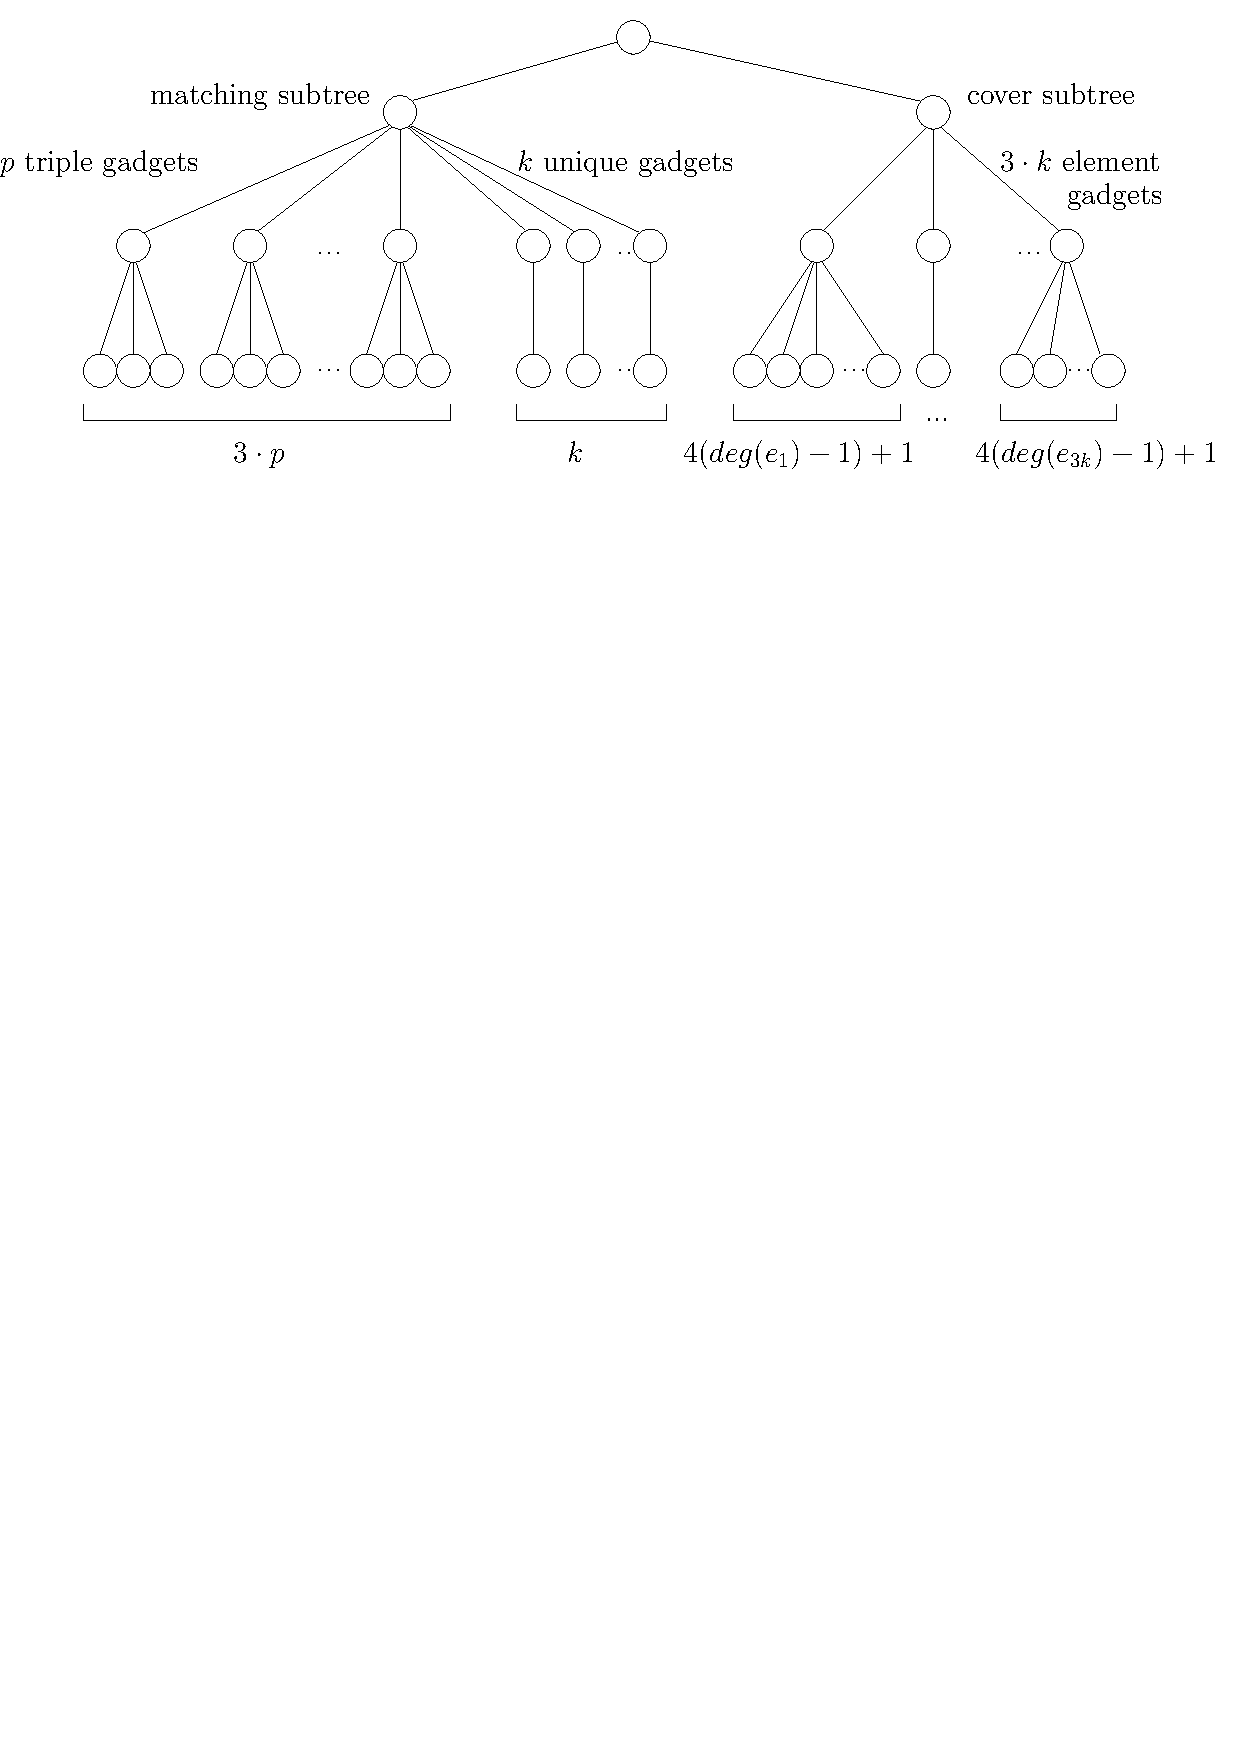
\includegraphics[width=0.9\columnwidth]{figs/static-mapping/overview}
  \caption{Overview of the substrate network in the proof of the NP-hardness of $\FP+\RS(2)+\MA$ variant of $\CTE$.}
  \label{fig:red-ma2}
\end{figure}


%We have seen that replica selection flexibility can render embeddings computationally hard.
Now we provide a more detailed look at this hardness result
and explore the minimal requirements for rendering replica selection hard.
Concretely, we show that already two replicas for each chunk are sufficient for computational intractability.

% We now show that the 2-replica selection variant is even NP-hard
%without capacity constraints.  In particular, we consider the 
%variant~$\RS(2)+\MA(4)+\FP$ with at most two replicas of each chunk and assignment factor
%four. There are no capacity constraints on links.
%
%Our construction consists of two major modifications to hardness result without replication factor restrictions (for that result, refer to Section~\ref{ssec:fprsma}).
%
%\parag{Unique chunks on the comb.} First, we provide the tools for restricting the placement of nodes in certain parts of the tree.
%In Section~\ref{ssec:fprsma}, due to symmetric structure of the tree, the carefully crafted threshold value allowed us to prove that e.g. no Triple Gadget ever had two or more nodes placed in it.
%We still use the threshold value as the placement mechanism, but in this section, due to the asymmetrical tree construction, we combine it with the concept of unique chunks on the comb (by \emph{comb} we denote the balanced tree, where all non-root vertices have at most one child).
%
%For an introduction to the concept of unique chunks, let us consider the following example.
%Suppose that within one $\VCEMB$ construction, we would like to encode not one $\TDPM$ instance, but two $\TDPM$ instances: $M_1$ and $M_2$, with disjoint universe and different number of triples to be chosen: $n_1$ and $n_2$.
%We perform the following modifications to the encoding provided in Section~\ref{ssec:fprsma}.
%The multi-assignment factor grows by $1$, that is the instance we construct is the $\RS+\MA(4)+\FP$ variant instance.
%We construct two subtrees $T_1$ and $T_2$, that correspond to $M_1$, resp. $M_2$; we construct two two-edge-level combs $C_1$ and $C_2$, with number of leaves $n_1$, resp. $n_2$.
%We attach $M_1$ and $C_1$ (resp. $M_2$ and $C_2$) to the common root and we name the resulting subtree $P_1$, resp. $P_2$.
%Next, we attach $P_1$ and $P_2$ to the common root.
%In the end, the height of the tree grew by $2$.
%Finally, we populate both combs with unique chunks, and we set the number of to-be-placed nodes to $\Vms = n_1+n_2$.
%We modify the threshold to be the sum of the thresholds for constructions for $M_1$ and $M_2$ plus $4\cdot (n_1 + n_2)$.
%The last substrate of the threshold value corresponds to transportation of the fourth chunk processed by each machine for the distance of four.
%
%To see why the example indeed can solve two instances of $\TDPM$, we need the following observations.
%First, we claim that no node is ever placed in a comb.
%To prove this fact, we use the property of the comb that the leaves are highly separated, and the fact that each machine has to process $4$ chunks.
%Next, we claim that the number of nodes placed in $P_1$ (resp. $P_2$) is $n_1$ (resp. $n_2$).
%To see this, consider any imbalance of the number of placed nodes; notice that some chunks in the underpopulated comb are processed outside of their $P_i$ subtree, resulting in the solution that exceeds the threshold.
%
%\parag{Families of chunks.} The second tool that we introduce allows us to express the redundancy of chunks without actually replicating chunks more than two-fold.
%For simplicity of introduction, we consider the scenario with no multi-assignment.
%For each chunk $c$ with redundancy, we count the number of occurrences of replicas of such a chunk in the tree, and name it $r_c$.
%We replace the chunk $c$ with $r$ chunks, which we call the family $F_c$ of that chunk.
%For each occurrence of replica of $c$, we replace it with a replica of any chunk from the family (without repetitions).
%To this point, the redundancy factor was reduced from $r_c$ to $1$.
%Now, we construct the gadget $G_c$ for chunk $c$, which consists of $r_c$ leaves, each hosting the second replica of each chunk from family $F_c$.
%We use the technique of unique chunks on the comb to constraint the number of nodes in $G_c$ to be exactly $r_c - 1$.
%We provide necessary additional $r_c-1$ nodes to be placed.
%Hence, exactly $1$ node is placed on a chunk of family $F_c$ outside the gadget $G_c$, and exactly $r_c-1$ nodes cover the remaining $r_c-1$ chunks inside gadget $G_c$.
%All chunks are processed, the replication factor is reduced to $2$, and the size of construction grows polynomially.

%\parag{Introduction to the reduction.} As we already stated, we modify the construction from Section~\ref{ssec:fprsma}.
%As a way to deal with replication, we use the families of chunks using the unique chunks on the comb.
%We extend the construction of a gadget for chunk with redundancy, by incorporating the fact that the multi-assignment factor is $4$.
%For the construction to remain correct given such a multi-assignment factor, we introduce further chunks with one chunk replica to place in the chunk gadget and use the excessive $3$ data processing capacities.

For an arbitrary instance~$\ITDPM$ of the~$\TDM$ problem, we construct a~$\RS(2)+\MA+\FP$ variant instance~$\ICTE$ the following way.
Let $k = |X|=|Y|=|Z|$ and $p = |P|$.
For each element $e\in X\cup Y\cup Z$, by $P_e$ we denote the set of all triples that contain $e$.
Let $\deg(e) = |P_e|$, and note that $\sum_e \deg(e) = 3\cdot p$.
We proceed with the construction as follows.
\paragraph{Substrate network.}
We construct a substrate network that consists of two subtrees connected to the
  root: a \emph{\MatchSubtree} and a \emph{\CoverSubtree}. The
  {\MatchSubtree} consists of $p$ \emph{\TripleGadgets} (one per each triple from $P$) and $k$
  \emph{\UnqGadgets}. The {\CoverSubtree} consists of~$3\cdot k$ \emph{\ElGadgets} $G(e)$, one for each element $e\in X\cup Y\cup Z$.
  The construction is depicted in Figure~\ref{fig:red-ma2}. Gadgets are constructed in the following way.
\begin{enumerate}
  \item Each {\TripleGadget} consists of four vertices: three leaves and the root of the gadget, as defined in the reduction for the $\FP+\RS+\MA$ variant in Section~\ref{ssec:fprsma}.
  \item Each {\UnqGadget} consists of two vertices: the leaf and the root of the gadget.
  This keeps the tree balanced, and also keeps leaves of
  {\UnqGadgets} far from each other.
  \item The {\ElGadget} $G(e)$ for element $e$ consists of the
  root and~$4\cdot(\deg(e)-1)+1$ leaves. There are $3\cdot k$ elements numbered from $e_1$ to $e_{3\cdot k}$, and $3\cdot k $ corresponding element gadgets $G(e_1), \ldots, G(e_{3\cdot k})$.
\end{enumerate}

\paragraph{Chunks.}
We construct three sets of chunks.
The first set corresponds to elements of the universe $X\cup Y\cup Z$.
This time we cannot repeat the construction of chunks from Section~\ref{ssec:fprsma}, because we need to obey the restricted replication factor.
%Namely, for each element of universe $e \in X \cup Y \cup Z$, we construct $\deg(e)$ chunks, each having two replicas.
%The set of $k$ \emph{unique} chunks is placed in the unique subtree and their role is to enforce the placement of exactly $k$ nodes in the matching subtree.
%We place $3\cdot(\deg(e) - 1)$ \emph{dummy} chunks in the element gadgets; each node in the element subtree needs to processes only $1$ element chunk and remaining $3$ of $\MaFactor=4$ chunks are the dummy chunks.
%Unique and dummy chunks have one replica, and we simply identify the chunk with chunk replica.
\begin{enumerate}
  \item \emph{Element chunks}. For each triple $t = \langle x, y, z \rangle \in P$, we construct $3$ chunks:~$x_t, y_t,$ and $z_t$, i.e., $\sum_e\deg(e)$ $=3\cdot p$ chunks in total.
  Each element $e$ have then $\deg(e)$ element chunks~$e_t$ for each $t \in P_e$,  collectively called $C_e$.
  Each chunk from $C_e$ have two replicas. First replicas are placed in the matching subtree:
  we place
  three replicas: $x_t^{(1)}, y_t^{(1)}$ and $z_t^{(1)}$ in the {\TripleGadget} for triple $t\in P$, one per each leaf.
  Second replicas are placed in the cover subtree:
  for each element $e \in X\cup Y\cup Z$, for each $t \in P_e$,
  we place replicas $e_t^{(2)}$ in different leaves of the gadget $G(e)$.
  In total, we place $\deg(e)$ replicas of element chunks in the leaves of the gadget $G(e)$.
  An example for $\TDPM$ instance from Figure~\ref{fig:fprsma} is given in Figure~\ref{fig:example-rs2}.
  \item \emph{Unique chunks}. We construct~$k$ unique chunks $u_1, \ldots, u_k$ with one replica each, and we place these replicas at the leaves of {\UnqGadgets} (one chunk per leaf).
  \item \emph{Dummy chunks}. For each element~$e\in X\cup Y\cup Z$,
  we construct an additional set of $3\cdot(\deg(e) - 1)$ dummy chunks, with one replica each, and we place these replicas in $3\cdot (\deg(e)-1)$ leaves of $G(e)$ (one chunk per leaf),
  not occupied by (the second) replicas of element chunks.
  Recall that the remaining $\deg(e)$ leaves of $G(e)$ contain replicas $e_t^{(2)}$ for each $t \in P_e$, i.e., one replica at each leaf.
\end{enumerate}

\begin{figure}[t]
\centering
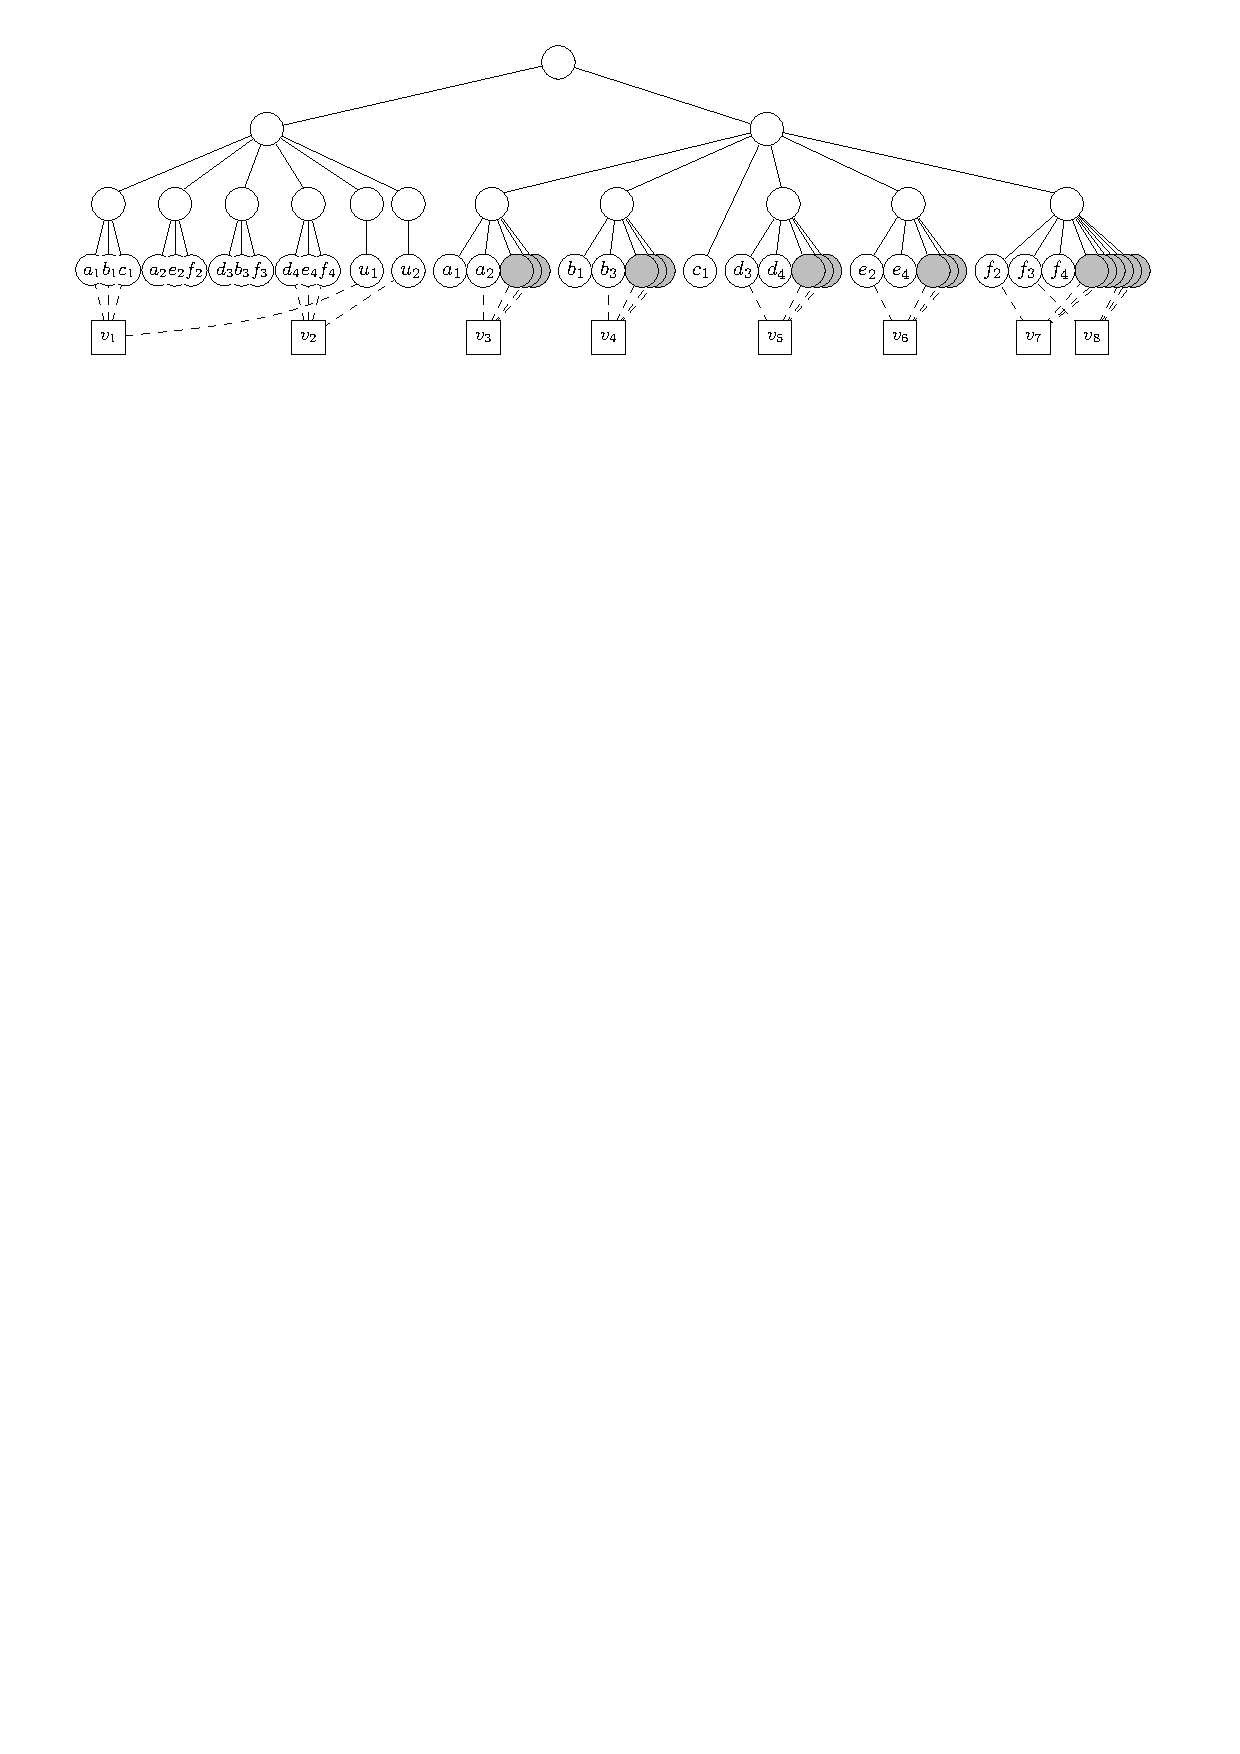
\includegraphics[width=1\columnwidth]{figs/static-mapping/cte-ma2.pdf}
\caption{An instance of $\FP+\MA+\RS(2)$ variant of $\CTE$ corresponding to the $\TDM$ instance from Figure~\ref{fig:fprsma}. Leaves containing dummy chunks are grey. The optimal solution assigns chunks to nodes $v_1, \ldots v_7$ by the dashed lines. In specifying the chunk placement we omit the replica superscripts.}
\label{fig:example-rs2}
\end{figure}


\paragraph{Other properties of the instance.}
The multi-assignment factor is $m=4$, and the number of nodes to embed is~$\numNodes = k + \sum_{e}(\deg(e)-1) = k + \sum_{e}\deg(e)-3\cdot k = 3\cdot p - 2\cdot k$.
 We set the cost threshold to~$\Thr = 8\cdot k + 6\cdot(n_V-k) = 18\cdot p - 10\cdot k$.

%\parag{The reduction.}
%Given any $\TDPM$ instance $\ITDPM$, we produce the corresponding instance $\ICTE$ of the $\RS(2)+\MA+\FP$ variant, in the way described above.
%The reduction (Theorem~\ref{th:ma-reduction}) consists of two parts.
%First, given a solution $\STDPM$ to $\ITDPM$, we construct a solution $\SCTE$ to $\ICTE$.
%This simply consists of placing nodes in triple gadgets for triples chosen in $\STDPM$.
%Next, given $\SCTE$, we construct the $\STDPM$.
%In this part, the main difficulty lies in showing that $\SCTE$ has certain structure.

 \bigskip
 
 Given any $\TDPM$ instance $\ITDPM$, we produce the corresponding instance $\ICTE$ of the $\RS(2)+\MA+\FP$ variant, in the way described above.
 We illustrate an instance of $\CTE$ corresponding to a $\TDPM$ instance from Figure~\ref{fig:fprsma} in Figure~\ref{fig:example-rs2}.
 The reduction (Theorem~\ref{th:ma-reduction}) consists of two parts: (1)~given a solution for $\ITDPM$, we construct a solution to $\ICTE$ of cost at most $\Thr$, and (2) given a solution for $\ICTE$ of cost at most $\Thr$, we construct a solution for $\ITDPM$.
 The first part is easier, and we present it now.
\begin{lemma}
  Fix an instance $\ITDPM$ of~$\TDPM$ and construct an instance $\ICTE$ of $\CTE$ in the way described in this section.
  If there exists a perfect 3D matching for $\ITDPM$, then $\ICTE$ has a~solution of cost at most $\Thr$.
    \label{lem:ma-reduction-left}
\end{lemma}
\begin{proof}
  Fix a feasible solution~$\STDPM$ for $\ITDPM$. We construct a solution~$\SCTE$ for $\ICTE$ in the following way:
  We place $n_V = k + \sum_e(\deg(e) - 1)$ nodes, and we assign $4$ chunks to each of these.
  \begin{enumerate}
    \item We place~$k$ nodes in~$k$ {\TripleGadgets} (one per gadget, at an arbitrary leaf) that correspond to triples chosen in~$\STDPM$ solution.
    To each such node we assign $3$ chunk replicas from its gadget and one arbitrary, unassigned unique chunk.
    \item For each element $e$, in $G(e)$ we place~$\deg(e) - 1$ nodes, and to each of them we assign $3$~arbitrary dummy chunks and $1$ replica of an arbitrary 
    element chunk (in this
    gadget) whose another replica is not assigned in any {\TripleGadget}.
    We co-locate the node with one of its assigned replicas, hence one of the assignments is for free, and other three assignments incur the cost $2$~each.
  \end{enumerate}
  Triples in $\STDPM$ match each element exactly once,
  and hence nodes in triple gadgets have exactly one chunk assigned from $C_e$ for each element $e$.
  For each element $e$, by $e_*$ we denote the element chunk $e_t$ that is assigned in a triple gadget, i.e, the replica $e_*^{(1)}$ is assigned in a triple gadget.
  The remaining $\deg(e)-1$ chunks from $C_e \setminus \{ e_* \}$ (their second replicas) are assigned to $\deg(e)-1$ nodes in $G(e)$.
  Finally, each of $k$ unique chunks is assigned to a~node in a triple gadget, and each dummy chunk is assigned to some node in its element gadget.
  
 % \todo{todo: explain: every chunk was processed}
  %Every chunk was assigned, exactly $n_V = k + \sum_e(\deg(e) - 1)$ nodes are placed, and each of the nodes has exactly $4$ chunk replicas assigned.
  To see that the solution does not exceed the threshold $\Thr$, we sum up the total assignment cost.
  The $k$ nodes placed in \TripleGadgets{} have three assignments to chunk replicas within the \TripleGadget{} of the total cost $0+2+2=4$, and one assignment of cost $4$ (to some \UnqGadget{}).
  The remaining $\Vms-k$ nodes placed in the \CoverSubtree{} have four assignments within element gadgets for the total cost $0+3\cdot 2 = 6$.
  Summing up, the incurred cost is $8\cdot k + 6\cdot (\Vms - k) = \Thr$, i.e., the solution is feasible.
\end{proof}

To construct a solution for $\ITDPM$ from a solution to $\ICTE$, we show that every feasible solution for $\ICTE$ has certain structure.
We call a {\TripleGadget} \textit{active}, if it contains a~single node at one of its leafs, and we call the node \textit{active} if it is placed in a {\TripleGadget}.
In the lemmas below, we show that in feasible solutions to $\ICTE$, exactly $k$ \TripleGadgets{} are active (similar to Theorem~\ref{th:ma-unlimited}).
In the instance $\ICTE$, chunks can be assigned to nodes at distance $0, 2, 4$ or $6$.
We call the assignments at distance $0$ or $2$ \emph{short}, and the ones at distance $4$ or $6$ \emph{long}.


  \begin{lemma}
    Any solution to $\ICTE$ with more than $k$ long assignments is infeasible.
    \label{lem:infeasible}
  \end{lemma}
  \begin{proof}
    Consider a solution that uses $k+i$ long assignments for $i>0$.
    The solution consists of $\MaFactor \cdot n_V = 4\cdot n_V$ assignments, and $k+i$ of them incur cost at least $4\cdot (k+i)$.
    As every leaf of the substrate network of $\ICTE$ contains one replica, at most $n_V$ assignments are free.
    As the minimum distance between leaves is $2$, the remaining $3\cdot n_V - k-i$ assignments incur the cost $2$ each.
    In total, the cost of the solution is then $4\cdot (k+i) + 2\cdot (3\cdot n_V - k-i) = 6\cdot n_V + 2\cdot k + 2\cdot i = \Thr + 2\cdot i$, i.e., the solution cost exceeds the threshold $\Thr$.
  \end{proof}

  
\begin{lemma}
  Any feasible solution to $\ICTE$ places exactly $k$ nodes in the \MatchSubtree.
  \label{lem:n-matchsubtree-ma}
\end{lemma}

\begin{proof}
  First, we show that at most $k$ nodes are placed in the \MatchSubtree.
  Each node placed in the \MatchSubtree{} has at most $3$ leaves in the distance at most $2$, hence at least one of its $\MaFactor=4$ assignments is long.
  Therefore, more than $k$ nodes in the matching subtree would lead to more than $k$ long assignments, and by Lemma~\ref{lem:infeasible}, the solution would be infeasible.
  
  As at most $k$ nodes are placed in the \MatchSubtree{}, at least $\Vms-k$ nodes are placed in the \CoverSubtree.
  Now we claim that the cover subtree contains exactly $n_V-k$ of them.
  Suppose the contrary, i.e., that $\Vms-k+i$ nodes were placed in the \CoverSubtree{} for $i > 0$.
  With each element gadget $G(e)$ we associate its \emph{volume} $\deg(e) - 1$.
  The volume corresponds to the maximum number of nodes that can be placed inside the gadget without causing a long assignment.
  If the number of nodes in $G(e)$ exceeds its volume, i.e., $\deg(e) - 1 + j_e$ nodes are placed in $G(e)$ for $j_e > 0$,
  then the number of chunks assigned to these nodes is $4\cdot (\deg(e) - 1 + j_e)$, and at most $4\cdot (\deg(e) - 1) + 1$ can be assigned within the gadget $G(e)$.
  For the remaining $4\cdot j_e - 1 \geq 3\cdot j_e$ chunks, long assignments are used.
  By the pigeon-hole principle, at least $i = \sum_e j_e$ nodes surpass the volume of their gadgets, causing at least $3\cdot i$ long assignments.
  As each of $k-i$ nodes in the matching subtree result in one long assignment, in total we have at least $k+2\cdot i$ long assignments and by Lemma~\ref{lem:infeasible}, the solution is infeasible, a~contradiction.
\end{proof}

\begin{lemma}
  A feasible solution $\SCTE$ to $\ICTE$ has no nodes placed in unique gadgets.
  \label{lem:no-unq-ma}
\end{lemma}
\begin{proof}
  By Lemma~\ref{lem:n-matchsubtree-ma}, exactly $k$ nodes were placed in the \MatchSubtree{}.
  Suppose that $j>0$ of these nodes were placed in the \UnqGadgets{}.
  Every leaf of every unique gadget is at distance at least $4$ from every other leaf of the substrate network.
  Hence, each of $j$ nodes placed in a unique gadget has at least $3$ out of its $\MaFactor = 4$ chunks assigned by a long assignment.
  As triple gadgets consists of $3$ leaves, each of remaining $k-j$ nodes placed in the triple gadget uses at least $1$ long assignment.
  In total, the number of long assignments would be then at least $k-j + 3\cdot j > k$, which by Lemma~\ref{lem:infeasible} would lead to infeasibility of $\SCTE$.
\end{proof}

\begin{lemma}
  In a feasible solution $\SCTE$ to $\ICTE$, exactly $k$ triple gadgets are active.
  \label{lem:n-active-ma}
\end{lemma}
\begin{proof}
  By Lemma~\ref{lem:n-matchsubtree-ma}, exactly $k$ nodes were placed in the \MatchSubtree{}.
  By Lemma~\ref{lem:no-unq-ma}, these $k$~nodes are placed in the triple gadgets and not in the unique gadgets.
As there are exactly $3$ replicas in each \TripleGadget{}, placing more than one node in a single \TripleGadget{} causes at least additional $3$ long assignments (the argument is the same as in the proof of Theorem~\ref{th:ma-unlimited}).
Therefore, exactly $k$ \TripleGadgets{} are active.
\end{proof}

\begin{lemma}
  In a feasible solution $\SCTE$ to $\ICTE$, the unique chunks are assigned by long assignments at distance 4, and remaining chunks are assigned by short assignments (at distance 0~or~2).
  \label{lem:short-ma}
\end{lemma}
\begin{proof}
  By Lemma~\ref{lem:infeasible}, in $\SCTE$ there are at most $k$ long assignments.
  By Lemma~\ref{lem:no-unq-ma}, these $k$~long assignments are depleted by $k$ unique chunks, and remaining chunks are assigned by short assignments.


  Now we show that the unique chunks are assigned at distance $4$ (and not at distance $6$).
  In total, we have $4\cdot n_V = 12\cdot p - 8\cdot k$ assignments.
  At most $n_V = 3\cdot p - 2\cdot k$ of these are for free, as a~node can be co-located with at most one replica.
  The $k$ unique chunks are assigned for the cost at least $4$ each, and the remaining $4\cdot n_V - k - n_V = 9\cdot p - 7\cdot k$ assignments incur cost at least $2$ each.
  Suppose that a unique chunk is assigned at distance $6$, i.e., the cost of assignment of the unique chunks is $4\cdot k + 2$.
  Then, the solution cost is $2\cdot(9\cdot p - 7\cdot k) + 4\cdot k + 2 = 18\cdot p - 10\cdot k + 2 = \Thr + 2 > \Thr$, i.e., the solution cost exceeds the threshold, a contradiction.
\end{proof}

\begin{lemma}
  In a feasible solution $\SCTE$ to $\ICTE$, each node in the matching subtree is assigned to one unique chunk and three chunks that are placed in the triple gadget the node is located at.
  \label{lem:one-unique-per-node}
\end{lemma}
\begin{proof}
  By Lemmas~\ref{lem:n-matchsubtree-ma} and \ref{lem:no-unq-ma}, $k$ nodes in the matching subtree are placed in triple gadgets.
  As triple gadgets have at most $3$ leaves, each of these nodes causes at least one long assignment.
  If a node had $i>1$ unique chunks assigned, then the total number of long assignments would be at least $k-1+i>k$, and by Lemma~\ref{lem:infeasible} the solution would be infeasible.
  If a node had $0$~unique chunks assigned, it would still cause a~long assignment.
  By Lemma~\ref{lem:short-ma}, each of $k$ unique chunks causes a~long assignment, and in total we would have at least $k+1$ long assignments,  and by Lemma~\ref{lem:infeasible} the solution would be infeasible.

  Remaining $3$ of $\MaFactor=4$ chunks assigned to each node in the matching subtree are assigned by the short assignment, and the only chunks in distance at most $2$ are the chunks located in the same gadget that the node is located at.
\end{proof}

\begin{theorem}
  The $\RS(2)+\MA+\FP$ variant of the $\CTE$ problem is NP-hard.
  \label{th:ma-reduction}
\end{theorem}

\begin{proof}
  
  Fix an instance $\ITDPM$ of~$\TDPM$.
  We show that~$\ICTE$ constructed on the basis of $\ITDPM$ has a solution of cost~$\leq \Thr$ if ($\Leftarrow$) and only if~($\Rightarrow$) $\ITDPM \in \TDPM$ (there exists a perfect 3D matching in $\ITDPM$).
  By Lemma~\ref{lem:ma-reduction-left}, ($\Leftarrow$) holds.

  To show ($\Rightarrow$), fix a feasible solution~$\SCTE$ for~$\ICTE$ in the way described in the construction section.
  By Lemma~\ref{lem:n-active-ma}, exactly $k$ \TripleGadgets{} are active.
  We construct the solution $\STDPM$ from the set of triples that correspond to active \TripleGadgets{}.

  Now, we show that $\STDPM$ is feasible, i.e., it matches every element of $X\cup Y\cup Z$ exactly once.
  By Lemma~\ref{lem:one-unique-per-node}, every active node is assigned to the three element chunks located at the gadget it is placed at.
  Hence, the chunks $x_t$, $y_t$ and $z_t$ assigned to an active node that corresponds to the triple $t = \langle x, y, z \rangle \in P$.
  
  For every element $e\in X\cup Y \cup Z$, we constructed chunks $C_e$, with two replicas each: one in the matching subtree and one in the cover subtree.
  Now we claim that in each element gadget $G(e)$, we assign exactly $\deg(e) - 1$ element chunks.
  Similar to the proof of Lemma~\ref{lem:n-matchsubtree-ma}, with each $G(e)$ we associate its volume.
  By Lemma~\ref{lem:n-matchsubtree-ma}, we place $n_V-k$ nodes in the cover subtree, i.e., the number of nodes equal the total volume of all gadgets $G(e)$.
  Hence, in each of $G(e)$ we have $n_e$ nodes, where $n_e$ is the volume of $G(e)$.
  In a single gadget $G(e)$, the total number of chunks is $4\cdot(\deg(e) - 1) + 1$, and nodes in this gadget have $4\cdot(\deg(e)-1)$ chunks assigned.
   The remaining $1$ element chunk is assigned in a triple gadget.
  Hence, the set of active nodes have $1$~of $\deg(e)$ element chunks assigned for each $e\in X\cup Y\cup Z$, and $\STDPM$ assigns each $e\in X\cup Y\cup Z$ exactly once.
 
%  Each of $3\cdot p = \sum_e \deg(e)$ element chunks has two replicas: one in the matching subtree and one in the cover subtree.
%  By Lemma~\ref{lem:one-unique-per-node}, $3\cdot k$ element chunks are matched in the matching subtree.
%  From Lemma~\ref{lem:n-active-ma}, $n_V - k = \sum_e (\deg(e) - 1)$ nodes are placed in the cover subtree.
%  Nodes in the cover subtree 
%
%  \todo{wyjasnij dokladniej i opisz tutaj strukture gadzetu element}
%  Chunks have two replicas; one replica is not processed in element gadget (indivisible argument).
%  The other replica is processed in the matching subtree by active nodes.
%\todo{uzyj 1 unique per node}
%  In total all are processed.
 % By Lemma~\ref{lem:infeasible}, we have at most $k$ long matches and,
%  by Lemma~\ref{lem:no-unq-ma}, all these long matches are depleted by $k$ unique chunks.
%  Therefore, all but the unique chunks are matched by a short match.
  
%  Therefore, each chunk $c(e, t)$ for each $e\in X\cup Y\cup Z$, for each $t \in P$ is matched by a short match.
%  Hence, each active node processes three chunks that are placed in its \TripleGadget, and collectively active nodes process $3 \cdot k$ chunks.


%  The number of chunks $4\cdot(\deg(e) - 1) + 1$ in each element gadget $G(e)$ is non-divisible by $\MaFactor = 4$, i.e.,
%  $4 | 4\cdot(\deg(e) - 1) + 1 = 1$.
%  As all matches in the element subtree are short, in each element gadget 
%  
%  Let $\tau(G(e)) = 4\cdot(\deg(e) - 1) + 1$ be the number of chunks placed in a gadget $G(e)$ for an element $e\in X\cup Y\cup Z$.
%  By construction, $4 | \tau(G(e)) = 1$.
%  Recall that all matches (besides unique chunks) are short.
%  Hence, in each $G(e)$, there exists a chunk $c(e, t)$ for some $t \in P$ that is not matched.
%  Let's call this chunk~$\Unmatched(e)$, and let~$\Unmatched := \cup_e \Unmatched(e)$.
%  Note that~$|\Unmatched| = 3\cdot k$.
%  The solution $\SCTE$ is feasible, hence every chunk is matched, and $\Unmatched(e)$ is covered by its second replica, placed in the matching subtree.
%  The set~$\Unmatched$ is covered by \ActiveNodes{}, and hence the set of triples in $\STDPM$ form a 3D Perfect Matching of $X\cup Y\cup Z$.
\end{proof}



\subsection{Hardness of Inter-connects}\label{ssec:fprscc}


%\subsubsection{Inter-connects with Unrestricted Number of Replicas}

Next, we prove that the joint optimization of node placement and replica selection
is NP-hard if an inter-connect has to be established between nodes.
In our terminology, this is the~$\FP+\RS+\NI$ variant.
The proof is similar in spirit to the proof of the~$\FP+\RS+\MA$ variant, however,
we modify the construction to account for the absence of~$\MA$:
we place a bandwidth constraints on the certain links in the substrate network.
Additionally, we choose
a high value for~$\CostTrans$ (the cost of chunk assignment), so that nodes are directly collocated with
their assigned chunks.
%We leverage the fact that any solution which does not
%assign zero or the maximum possible number of chunks to each gadget has higher communication costs.

\parag{Construction.}
Let~$\ITDPM$ be an instance of~$\TDM$ with $p$ triples and set cardinality $k = |X| = |Y| = |Z|$.
We use the identical substrate network as in Section~\ref{ssec:fprsma} with
identical chunk replicas placed in the same way.
This time, however, the inter-connect cost is~$\CostCom = 1$, and the number of nodes (virtual machines) is~$\Vms = 3 \cdot k$, where~$k$ is the set cardinality.
The threshold value is $\Thr := 6\cdot k + 18\cdot (k-1)\cdot k = 2\cdot (3\cdot k) + 4\cdot({ 3\cdot k \choose 2} - (3\cdot k))$, and we set the access cost~$\CostTrans$ to $\Thr + 1$.
High assignment cost forces each node to be collocated with the replica assigned to it.
%Intuitively, in order to minimize embedding costs,
%nodes should be placed in near-by leaves of the substrate network.
We formalize this observation in Lemma~\ref{lemma:helper}.
\begin{lemma}\label{lemma:helper}
In any feasible solution to~$\ICTE$, $k$ gadgets have exactly
$3$ nodes each, and~$p-k$ gadgets remain empty.
\end{lemma}
\begin{proof}
The~$n_V = 3\cdot k$ nodes have to be placed
directly at different $3\cdot k$ leaves, and thus at $3\cdot k$ chunks, as otherwise the access cost would immediately exceed the threshold $\Thr$.
The $3\cdot k$ nodes are distributed among at least $k$ gadgets, as each gadget can host at most $3$ nodes.
In total there are ${3\cdot k \choose 2}$ pairs of nodes,
and the inter-connect cost is $2$ for each intra-gadget pair and $4$ for each inter-gadget pair.
%Note that at most $3\cdot k$ intra-gadget pairs exist, as at most $3$ pairs of nodes exist in each gadget.
If a gadget contains $3$ nodes, then it has $3$ intra-gadget pairs, if it contains $2$ nodes, then it has $1$ intra-gadget pair, and it has $0$ of these otherwise.

Suppose that nodes were distributed among more than $k$ gadgets.
Then, some gadgets contain less than $3$ nodes, and the number of intra-gadget pairs is $3\cdot k - i$ for some $i>0$.
Hence, the total cost is then $2\cdot (3\cdot k - i) + 4 \cdot ({3 \cdot k \choose 2} - (3\cdot k - i)) = 6\cdot k + 4 \cdot ({3 \cdot k \choose 2} - 3\cdot k) + 2\cdot i = \Thr + 2\cdot i$, and the solution exceeds the threshold $\Thr$.
\end{proof}

\begin{theorem}
\label{theorem:fp_rs_cc}
The $\FP+\RS+\NI$ variant of $\CTE$ problem is NP-hard.
\end{theorem}
\begin{proof}
Let~$\ITDPM$ be the corresponding instance of~$\TDM$ and let~$\ICTE$ be an instance of
the~$\FP+\RS+\NI$ variant constructed as described above.
We prove that~$\ICTE$ has solution of cost~$\leq \Thr$ if ($\Rightarrow$) and only if
($\Leftarrow$)
$\ITDPM$ has a~solution.

($\Rightarrow$) To compute a solution
for~$\ICTE$ given a solution for~$\ITDPM$, we proceed as follows.
Given a perfect matching $\STDPM$ consisting of triples~$ \{t_1, t_2,
\ldots, t_k\}$, we place three nodes in each gadget that
corresponds to every triple of~$\STDPM$ (one node per leaf). Chunks are assigned to the nodes which are co-located
in the same server.

The solution has the following cost:
(1) the inter-connect cost inside each gadget is~${2 \cdot {3 \choose 2} = 6}$,
  as the~distance between every pair of nodes there is $2$;
  (2) the the inter-connect cost from a~single gadget to all other gadgets is~$4
  \cdot 3 \cdot 3 \cdot (k - 1) / 2 = 18\cdot (k-1)$, where the factor~$4$ corresponds to the distance $4$, the factor~$3$
  corresponds to the number of nodes per gadget, and~$3 \cdot (k-1)$ is the number of nodes in remote gadgets;
  as we count each pair twice, we need to divide by two.
Summing up over all~$k$ gadgets, the total cost is $6\cdot k + 18\cdot(k-1)\cdot k = \Thr$.

($\Leftarrow$) Given a solution for~$\ICTE$,
we use Lemma~\ref{lemma:helper} to construct a solution for~$\ITDPM$: in any solution of cost at most~$\Thr$,
$k$ gadgets contain exactly 3 nodes. These gadgets correspond to a~valid
3D Perfect Matching, as exactly one replica of every chunk is assigned and
hence every element is covered exactly once.
\end{proof}

\paragraph{Remark on two replicas and inter-connects.}
It is worth noting that the $\FP+\RS(2)+\NI+\BW$ variant is also NP-hard~\cite{my-tcs}.
The reduction uses similar construction to the reduction from Section~\ref{ssec:fprsma},
with the help of bandwidth constraints that allow to control the number of nodes placed in a subtree.

%%%%%%%%%%%%%%%%%%%%%%%%%%%%%%%%%%%%%
\section{Conclusions}\label{sec:conclusion-static}


In this chapter, we have shown that despite the
multiple dimensions of flexibility in terms of chunk assignment and node placement, 
and despite the large scale of modern data centers, 
many variants can be solved efficiently. However, we have also
shown that several embedding variants are NP-hard already in two-
and three-level trees---a practically relevant result given today's data center topologies~\cite{fattree}.


%\begin{table}
%\tiny
%\bgroup
%\def\arraystretch{1.5}
%\begin{small}
%\begin{tabular}{|l|l|p{6.5cm}|}
%\hline
%\multirow{3}{*}{NP-hard} & 5 combinations & \mbox{$\RS+\MA+\FP+\NI+\BW$}\\
%\cline{2-3}
% & 4 combinations &  \mbox{$\RS+\MA+\FP+\NI$}; \mbox{$\RS+\MA+\FP+\BW$};
%\mbox{$\RS+\FP+\NI+\BW$} \\ \cline{2-3}
% & 3 combinations &\mbox{$\RS+\MA+\FP$};~\mbox{$\RS+\FP+\NI$} \\
% \hline
% \hline
%\multirow{3}{*}{Flow} & 4 combinations & \mbox{$\RS+\MA+\NI+\BW$} \\ \cline{2-3}
% & 3 combinations & \mbox{$\RS+\NI+\BW$}; \mbox{$\RS+\MA+\BW$}    \\ \cline{2-3}
% & 2 combinations &$\RS+\BW$ \\
% \hline
% \hline
%\multirow{3}{*}{DP} & 4 combinations & \mbox{$\MA+\FP+\NI+\BW$} \\ \cline{2-3}
% & 3 combinations &   \mbox{$\MA+\FP+\NI$};
%\mbox{$\MA+\FP+\BW$}; \mbox{$\FP+\NI+\BW$} \\ \cline{2-3}
% & 2 combinations & \mbox{$\MA+\FP$};~\mbox{$\FP+\NI$}; \\
% \hline
% \hline
%\multirow{3}{*}{Matching} &3 combinations&
%\mbox{$\RS+\MA+\NI$};~\mbox{$\MA+\NI+\BW$}  \\
%\cline{2-3}
% & 2 combinations & \mbox{$\RS+\MA$};
%\mbox{$\RS+\NI$}; \mbox{$\MA+\NI$};
%\mbox{$\MA+\BW$}; \mbox{$\NI+\BW$} \\ \cline{2-3}
%& 1 combinations & \mbox{$\RS$}; \mbox{$\MA$};
%\mbox{$\NI$}; \mbox{$\BW$}\\
% \hline
% \hline
% \multirow{3}{*}{0 Cost} & 3 combinations & \mbox{$\RS+\FP+\BW$}\\
%\cline{2-3}
% & 2 combinations & \mbox{$\RS+\FP$}; \mbox{$\FP+\BW$}\\ \cline{2-3}
% & 1 combinations & \mbox{$\FP$}\\
% \hline
%\end{tabular}
%\end{small}
%\caption{
%Fastest algorithms for different respective problem variants.
%}
%\vspace{-2em}
%\label{tab:summary}
%\egroup
%\end{table}


Our results are summarized in
Figure~\ref{fig:venn_full}.
One interesting take away from this figure regards
the question which properties render the problem
NP-hard. For instance, we see that~$\BW$
does not influence the hardness of any variant,
while~$\RS$ is crucial for NP-hardness.
$\MA$ only affects hardness if combined with~$\RS$.
$\NI$ is trivial without~$\FP$, and~$\FP$ requires
more sophisticated algorithms when combined with~$\NI$ or~$\MA$;
in combination with~$\RS$ and~$\MA$ or~$\NI$,~$\FP$ renders the
problem NP-hard.
